% !TEX root = saveliev_physics_general_course_2.tex
%!TEX TS-program = pdflatex
%!TEX encoding = UTF-8 Unicode


\chapter[TỪ TRƯỜNG TRONG CHÂN KHÔNG]{TỪ TRƯỜNG\\ TRONG CHÂN KHÔNG}\label{chap:6}
\chaptermark{TỪ TRƯỜNG TRONG CHÂN KHÔNG}

\section{Tương tác giữa dòng điện}\label{sec:6_1}
Thực nghiệm đã cho biết dòng điện có thể tác dụng lực lên nhau. Ví dụ, hai dây dẫn thẳng và tiết diện rất nhỏ đặt song song nhau và có dòng điện chạy qua sẽ hút nhau nếu dòng điện trong chúng chạy cùng chiều nhau, và đẩy nhau nếu dòng điện chạy ngược chiều nhau. Lực tương tác trên một đơn vị chiều dài của mỗi dây dẫn tỉ lệ thuận với các cường độ dòng điện $I_1$ và $I_2$ qua chúng và tỉ lệ nghịch với khoảng cách $b$ giữa chúng:
\begin{equation}\label{eq:6_1}
    \ab{F}{u} = k \frac{2 I_1 I_2}{b}.
\end{equation}

\noindent
Chúng ta sẽ làm rõ lí do tại sao lại đặt hệ số tỉ lệ là $2k$ trong các trang sau.

Định luật về tương tác giữa các dòng điện đã được thiết lập vào năm 1820 bởi nhà vật lý Andre Ampere (1775-1836). Biểu thức tổng quát cho mọi vật dẫn của định luật trên sẽ được giới thiệu ở \sect{6_6}. Biểu thức \eqref{eq:6_1} đã được sử dụng để quy ước đơn vị của cường độ dòng điện trong hệ SI và trong hệ đơn vị điện từ chuẩn (cgsm). Đơn vị SI của cường độ dòng điện---\textbf{ampere}---được định nghĩa là cường độ của dòng điện không đổi cần được cho chạy qua hai dây dẫn thẳng dài vô hạn, song song nhau, tiết diện không đáng kể và đặt trong chân không, cách nhau $1$ mét để lực tương tác giữa các dây dẫn trên là \num{2e-7} newton trên mét.

Đơn vị của điện tích, \textbf{coulomb}, được định nghĩa là lượng điện tích chạy qua tiết diện của một vật dẫn trong $1$ giây khi có dòng điện không đổi $1$ ampere. Vì vậy mà coulomb còn được gọi là \textbf{ampere-giây} (\si{\ampere\second}).

Phương trình \eqref{eq:6_1} được viết lại như sau:
\begin{equation}\label{eq:6_2}
    \ab{F}{u} = \frac{\mu_0}{4\pi} \frac{2 I_1 I_2}{b},
\end{equation}

\noindent
trong đó $\mu_0$ được gọi là \textbf{hằng số từ} [giống như \eqn{1_11}]. Để tính giá trị của $\mu_0$, chúng ta sẽ sử dụng định nghĩa của ampere: khi $I_1=I_2=\SI{1}{\ampere}$ và $b=\SI{1}{\metre}$, lực tương tác $\ab{F}{u}$ sẽ bằng \SI{2e-7}{\newton\per\metre}.

Thay các giá trị trên vào \eqref{eq:6_2}:
\begin{equation*}
    \num{2e-7} = \frac{\mu_0}{4\pi} \frac{2\times 1\times 1}{1}.
\end{equation*}

\noindent
Vậy,
\begin{equation}\label{eq:6_3}
    \mu_0 = 4 \pi \times \num{e-7} = \SI{1.26e-6}{\henry\per\metre}
\end{equation}

\noindent
(ký hiệu \si{\henry\per\metre} có nghĩa là henry trên mét---xem \sect{8_5}).

Hằng số $k$ trong biểu thức \eqref{eq:6_1} sẽ bằng 1 nếu ta chọn đơn vị phù hợp cho dòng điện. Đây là lí do vì sao hệ đơn vị điện từ chuẩn (cgsm$_I$) được thành lập. Trong hệ trên, đơn vị của dòng điện được định nghĩa là cường độ dòng điện cần được cho chạy qua dây dẫn thẳng dài vô hạn, tiết diện nhỏ để lực tác dụng lên một dây dẫn tương tự được đặt song song và cách nhau \SI{1}{\centi\metre} là $2$ dyn trên centimét của dây ($1$ dyn = \SI{e-5}{\newton})
 
Trong hệ cgse, hằng số $k$ là một đại lượng có thứ nguyên. Từ phương trình \eqref{eq:6_1}, thứ nguyên của $k$ được xác định là:
\begin{equation}\label{eq:6_4}
    [k] = \frac{[\ab{F}{u} b]}{[I]^2} = \frac{[F]}{[I]^2}.
\end{equation}

\noindent
Ta thấy rằng vì $\ab{F}{u}$ có thứ nguyên là lực chia chiều dài; vậy, thứ nguyên của tích $\ab{F}{u}b$ sẽ là thứ nguyên của lực. Từ \eqref{eq:1_7}\eqref{eq:5_7}:
\begin{equation*}
    [F] = \frac{[q]^2}{\text{L}^2};\quad [I] = \frac{[q]}{\text{T}}.
\end{equation*}

\noindent
Từ các giá trị ở \eqref{eq:6_4}, ta có được:
\begin{equation*}
    [k] = \frac{\text{T}^2}{\text{L}^2}.
\end{equation*}

\noindent
Vậy, trong hệ cgse, hằng số $k$ có thể viết là
\begin{equation}\label{eq:6_5}
    k = \frac{1}{c^2},
\end{equation}

\noindent
với $c$ là đại lượng có thứ nguyên vận tốc, gọi là \textbf{hằng số điện từ}. Để tìm giá trị của nó, chúng ta sẽ sử dụng liên hệ đã được thiết lập bằng thực nghiệm \eqref{eq:1_8} giữa coulomb và đơn vị cgse của điện tích. Lực \SI{2e-7}{\newton\per\metre} sẽ tương đương với \SI{2e-4}{\dyne\per\centi\metre}. Từ biểu thức \eqref{eq:6_1}, đây là lực tương tác giữa hai dòng điện có cường độ \num{3e9} \cgse{I} (\ie, \SI{1}{\ampere}) khi $b=\SI{100}{\centi\metre}$. Vậy,
\begin{equation*}
    \num{2e-4} = \frac{1}{c^2} \frac{2\times \num{3e9} \times \num{3e9}}{100},
\end{equation*}

\noindent
suy ra
\begin{equation}\label{eq:6_6}
    c = \SI{3e10}{\centi\metre\per\second} = \SI{3e8}{\metre\per\second}.
\end{equation}

Giá trị của hằng số điện từ bằng với vận tốc ánh sáng trong chân không. Từ lý thuyết của J. Maxwell, ta có thể thấy rằng sóng điện từ trong chân không có vận tốc bằng hằng số điện từ $c$. Sự trùng hợp giữa $c$ và vận tốc ánh sáng là cơ sở để Maxwell đoán rằng ánh sáng là một loại sóng điện từ.

Giá trị của $k$ trong biểu thức \eqref{eq:6_1} là $1$ trong hệ đơn vị cgsm và $1/c^2=1/\parenthesis{\num{3e10}}^2$ \si{\second\squared\per\centi\metre\squared} trong hệ đơn vị cgse. Vậy, dòng điện có cường độ $1$ cgsm$_I$ là tương đương với dòng có cường độ \num{3e10}\cgse{I}:
\begin{equation}\label{eq:6_7}
    1 \cgs{m}{I} = \SI{3e10}{\cgs{e}{I}} = \SI{10}{\ampere}.
\end{equation}

\noindent
Nhân 2 vế của liên hệ trên với \SI{1}{\second}, ta được
\begin{equation}\label{eq:6_8}
    1 \cgs{m}{q} = \SI{3e10}{\cgs{e}{q}} = \SI{10}{\coulomb}.
\end{equation}

\noindent
Vậy,
\begin{equation}\label{eq:6_9}
    \ab{I}{cgsm} = \frac{1}{c} \ab{I}{cgse}.
\end{equation}

\noindent
Tương tự,
\begin{equation}\label{eq:6_10}
    \ab{q}{cgsm} = \frac{1}{c} \ab{q}{cgse}.
\end{equation}

Tồn tại mối liên hệ giữa các hằng số $\varepsilon_0$, $\mu_0$, và $c$. Để thiết lập liên hệ trên, chúng ta sẽ tìm thứ nguyên và giá trị số của tích $\varepsilon_0\mu_0$. Từ phương trình \eqref{eq:1_11}, đơn vị của $\varepsilon_0$ là
\begin{equation}\label{eq:6_11}
    [\varepsilon_0] = \frac{[q]^2}{\text{L}^2 [F]}.
\end{equation}

\noindent
Từ \eqref{eq:6_2}
\begin{equation}\label{eq:6_12}
    [\mu_0] = \frac{[\ab{F}{u} b]}{[I]^2} = \frac{[F] \text{T}^2}{[q]^2}.
\end{equation}

\noindent
Nhân hai biểu thức \eqref{eq:6_11}\eqref{eq:6_12} cho ta
\begin{equation}\label{eq:6_13}
    [\varepsilon_0\mu_0] = \frac{\text{T}^2}{\text{L}^2} = \frac{1}{[v]^2}
\end{equation}

\noindent
($v$ là tốc độ).

Dựa trên các phương trình \eqref{eq:1_11} và \eqref{eq:6_3}, giá trị của tích $\varepsilon_0\mu_0$ là
\begin{equation}\label{eq:6_14}
    \varepsilon_0\mu_0 = \frac{1}{4 \pi \times \num{9e9}} \times 4\pi \times \num{e-7} = \frac{1}{\parenthesis{\num{3e8}}^2}\, \si{\second\squared\per\centi\metre\squared}.
\end{equation}

Cuối cùng, từ các phương trình \eqref{eq:6_6}, \eqref{eq:6_13}, và \eqref{eq:6_14}, chúng ta sẽ rút ra được mối liên hệ rất thú vị sau:
\begin{equation}\label{eq:6_15}
    \varepsilon_0\mu_0 = \frac{1}{c^2}.
\end{equation}

\section{Từ trường}\label{sec:6_2}

Dòng điện tương tác với nhau thông qua \textbf{từ trường}. Vào năm 1820, nhà vật lý học người Đan Mạch Hans Oersted (1777-1851) đã phát hiện ra ảnh hưởng của dòng điện lên nam châm. Oersted đã đặt một kim la bàn bên dưới dây dẫn có dòng điện chay qua. Khi dòng được bật lên, kim la bàn luôn xoay sao cho hướng của nó vuông góc với hướng của dây. Nó sẽ quay ngược lại nếu chúng ta đảo chiều dòng điện.

Thí nghiệm của Oersted đã cho thấy từ trường có hướng và do đó, phải được biểu diễn bằng một đại lượng vector. Chúng ta kí hiệu đại lượng trên là $\vec{B}$. Sẽ hợp lí nếu chúng ta gọi $\vec{B}$ là cường độ từ trường, giống như với cường độ điện trường $\vec{E}$. Tuy nhiên, vì các lí do về lịch sử phát hiện nên chúng ta sẽ gọi $\vec{B}$ là \textbf{cảm ứng từ}. Thay vào đó, chúng ta đặt tên cường độ từ trường cho đại lượng thứ cấp $\vec{H}$ , giống như đại lượng thứ cấp $\vec{D}$ của điện trường.

Không như điện trường, từ trường chỉ tác dụng lực lên các điện tích chuyển động. Các điện tích đứng yên không chịu ảnh hưởng của từ trường.

Một vật dẫn có dòng điện là một hệ trung hòa điện, trong đó một loại điện tích sẽ chuyển động theo một hướng và loại còn lại sẽ chuyển động ngược lại (hoặc đứng yên). Từ đây, ta suy ra rằng từ trường được sinh ra bởi các điện tích chuyển động.

Vậy, điện tích chuyển động (dòng điện) thay đổi tính chất của không gian xung quanh nó---bằng cách sinh ra từ trường. Trường trên tương tác với các điện tích chuyển động (dòng điện) bằng cách tác dụng lực lên chúng.

Thực nghiệm đã cho thấy nguyên lý chồng chập vẫn đúng cho từ trường, giống như điện trường: \textit{trường $\vec{B}$ được sinh ra từ nhiều điện tích chuyển động (dòng điện) là tương đương với tổng vector của các trường $\vec{B}_i$ do từng điện tích chuyển động (dòng điện) sinh ra:}
\begin{equation}\label{eq:6_16}
    \vec{B} = \sum_i \vec{B}_i
\end{equation}

\noindent
[giống với \eqn{1_19}].

\section{Từ trường của Điện tích chuyển động}\label{sec:6_3}

Vì không gian là đẳng hướng nên nếu điện tích đứng yên thì tất cả các phương bình đẳng.   Đây là lí do tại sao điện trường tĩnh của điện tích điểm là đối xứng cầu.

Khi một điện tích điểm di chuyển với vận tốc $\vec{v}$, một hướng được ưu tiên sẽ xuất hiện trong không gian (hướng của vector $\vec{v}$). Do đó, chúng ta có thể dự đoán rằng từ trường của điện tích chuyển động sẽ có đối xứng trục. Lưu ý rằng ở đây chúng ta đang xem xét chuyển động tự do của điện tích \ie, chuyển động với vận tốc không đổi. Để xuất hiện gia tốc, điện tích phải chịu ảnh hưởng của một trường nào đó (điện trường hoặc từ trường). Sự tồn tại của trường này sẽ phá vỡ tính đẳng hướng của không gian.

Chúng ta sẽ xem xét từ trường ở điểm $P$ bởi điện tích $q$ chuyển động với vận tốc $\vec{v}$ (\fig{6_1}). Các xáo động trong không gian được truyền từ điểm này sang điểm kia với vận tốc giới hạn $c$. Vì lý do này, cảm ứng từ $\vec{B}$ tại điểm $P$ ở thời điểm $t$ không được xác định bởi vị trí của điện tích ở $t$ mà bởi vị trí của điện tích ở một thời điểm trước đó $t-\tau$:
\begin{equation*}
    \vec{B}(P,t) = f\{q, \vec{v}, \vec{r}(t-\tau)\}.
\end{equation*}

\noindent
Ở đây, $P$ là kí hiệu của các tọa độ của điểm $P$ được xác định trong hệ quy chiếu đứng yên, và $\vec{r}(t-\tau)$ là vector vị trí nối tới điểm $P$ từ vị trí của điện tích trong quá khứ, ở thời điểm $t-\tau$.

\begin{figure}[t]
	\begin{center}
		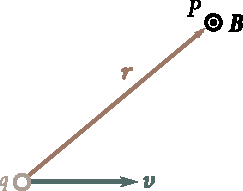
\includegraphics[scale=1]{figures/ch_06/fig_6_1.pdf}
		\caption[]{}
		\label{fig:6_1}
	\end{center}
	\vspace{-0.8cm}
\end{figure}

Nếu vận tốc của điện tích điểm nhỏ hơn đáng kể so với $c$ ($v\ll c$) thì thời gian trễ $\tau$ sẽ rất nhỏ. Khi đó, chúng ta có thể coi rằng giá trị của $\vec{B}$ tại thời điểm $t$ sẽ được quyết định bởi vị trí của điện tích điểm vào cùng thời điểm $t$. Nếu điều kiện trên thỏa mãn thì
\begin{equation}\label{eq:6_17}
    \vec{B}(P,t) = f\{q, \vec{v}, \vec{r}(t)\}
\end{equation}

\noindent
[ta thấy rằng vì $\vec{v}=\text{constant}$ nên $\vec{v}(t-\tau)=\vec{v}(t)$].

Hàm ở \eqref{eq:6_17} chỉ có thể được xác lập bằng thực nghiệm. Tuy nhiên, trước khi xem xét kết quả thí nghiệm, chúng ta sẽ thử tìm dạng hợp lí nhất của hệ thức trên. Giả thiết đơn giản nhất là độ lớn của $\vec{B}$ tỉ lệ thuận với điện tích $q$ và vận tốc $v$ (khi $\vec{v}\to 0$, từ trường biến mất). Chúng ta phải thiết lập vector $\vec{B}$ từ đại lượng vô hướng $q$ và hai vector $\vec{v}$ và $\vec{r}$. Chúng ta có thể lấy tích vector của hai vector trên rồi nhân chúng với đại lượng vô hướng. Khi đó, ta sẽ có biểu thức sau
\begin{equation}\label{eq:6_18}
    q (\vecprod{v}{r}).
\end{equation}

\noindent
Độ lớn của đại lượng trên tăng khi đi xa khỏi điện tích (tăng $r$). Khó có thể tồn tại một trường với tính chất như vậy---với tất cả các trường mà chúng ta đã biết đến (tĩnh điện, hấp dẫn), ta đều thấy rằng trường yếu đi khi đi xa khỏi nguồn, tỉ lệ thuận với $1/r^2$. Chúng ta sẽ giả sử rằng từ trường của điện tích chuyển động cũng thay đổi tương tự khi $r$ thay đổi. Khi đó, ta có thể đưa đại lượng trên về tỉ lệ với bình phương $r$ bằng cách chia \eqn{6_18} cho $r^3$. Kết quả là
\begin{equation}\label{eq:6_19}
    \frac{q (\vecprod{v}{r})}{r^3}.
\end{equation}

Thực nghiệm cho thấy rằng khi $v\ll c$, cảm ứng từ được sinh ra bởi điện tích chuyển động được xác định bởi công thức
\begin{equation}\label{eq:6_20}
    \vec{B} = k' \frac{q (\vecprod{v}{r})}{r^3},
\end{equation}

\noindent
trong đó $k'$ là hệ số tỉ lệ.

Chúng ta phải nhấn mạnh rằng các lập luận ta sử dụng để có được \eqref{eq:6_19} không nên được coi như cách chứng minh \eqn{6_20}. Các lập luận trên thiếu tính xác thực và mục đích chính của nó là để giúp chúng ta nhớ và hiểu \eqn{6_20}. Công thức trên chỉ có thể được chúng minh bằng thực nghiệm.

Từ \eqn{6_20}, ta có thể thấy rằng vector $\vec{B}$ tại mọi điểm $P$ đều có hướng vuông góc với mặt phẳng chứa vector $\vec{v}$ và điểm $P$, sao cho sự quay theo chiều của $\vec{B}$ tạo một tam diện thuận với hướng của $\vec{v}$ (xem kí hiệu hình tròn có dấu chấm ở giữa trong \eqn{6_1}). Lưu ý rằng $\vec{B}$ là một giả vector. Giá trị của hằng số tỉ lệ $k'$ phụ thuộc vào hệ đơn vị được sử dụng trong \eqn{6_20}. Biểu thức trên có thể được hữu tỷ hóa như sau:
\begin{equation}\label{eq:6_21}
    \vec{B} = \frac{\mu_0}{4\pi} \frac{q (\vecprod{v}{r})}{r^3}.
\end{equation}

\noindent
Ta có thể viết lại phương trình trên dưới dạng
\begin{equation}\label{eq:6_22}
    \vec{B} = \frac{\mu_0}{4\pi} \frac{q (\vec{v}\times\vecuni{r})}{r^3}
\end{equation}

\noindent
[có thể so với \eqn{1_15}]. Ta thấy rằng trong những biểu thức giống nhau giữa điện và từ mà có $\varepsilon_0$ trong mẫu số thì $\mu_0$ sẽ ở trong tử số và ngược lại.

Đơn vị SI của cảm ứng từ là \textbf{tesla} (\si{\tesla}) để vinh danh nhà phát minh người Croatia tên là Nikola Tesla (1856-1943).

Đơn vị của cảm ứng từ $B$ trong hệ đơn vị cgse và cgsm được chọn sao cho hằng số $k'$ trong \eqn{6_20} bằng 1. Do đó, mối liên hệ giữa các đơn vị của $B$ trong các hệ trên cũng giống như mối liên hệ giữa các đơn vị của điện tích:
\begin{equation}\label{eq:6_23}
    1 \cgs{m}{B} = \num{3e10} \cgs{e}{B}
\end{equation}

\noindent
[xem \eqn{6_8}].

Đơn vị của cảm ứng từ trong hệ cgsm có tên riêng---\textbf{gauss} (\si{\gauss}).

Nhà toán học người Đức Karl Gauss (1777-1855) đã đề xuất một hệ đơn vị trong đó tất cả các đại lượng liên quan đến điện (điện tích, dòng điện, cường độ điện trường, ...) đều được đo bằng hệ đơn vị cgse, và mọi đại lượng liên quan tới từ (cảm ứng từ, moment từ, etc.) đều được đo bằng hệ đơn vị cgsm. Hệ đơn vị kể trên được gọi là hệ đơn vị \textbf{Gaussian}, để tưởng nhớ người sáng tạo ra nó.

Trong hệ Gaussian, do \eqns{6_9}{6_10} mà mọi biểu thức chứa dòng điện hay điện tích sẽ được nhân thêm với $1/c$ ứng với mỗi đại lượng $I$ hay $q$ trong biểu thức đó. Hằng số được nhân thêm này giúp chuyển đổi giá trị của đại lượng liên quan ($I$ hay $q$) từ hệ đơn vị cgse sang hệ đơn vị cgsm (hệ đơn vị cgsm được thiết lập sao cho hệ số tỉ lệ trong mọi biểu thức bằng $1$). Ví dụ, trong hệ Gaussian, \eqn{6_20} có dạng là
\begin{equation}\label{eq:6_24}
    \vec{B} = \frac{1}{c} \frac{q (\vecprod{v}{r})}{r^3}.
\end{equation}

Ta thấy rằng sự xuất hiện của một hướng được ưu tiên trong không gian (hướng của vector $\vec{v}$) khi có điện tích chuyển động dẫn tới việc điện trường của điện tích trên mất đi đối xứng cầu và trở thành đối xứng trục. Các phép tính cho thấy các đường sức điện của điện trường sinh ra bởi điện tích chuyển động tự do sẽ có dạng như \fig{6_2}. Vector $\vec{E}$ tại điểm $P$ sẽ hướng theo vector vị trí $\vec{r}$ kẻ từ vị trí hiện tại của điện tích đến điểm $P$. Biểu thức của cường độ điện trường là
\begin{equation}\label{eq:6_25}
    E = \frac{1}{4\pi\varepsilon_0} \frac{q}{r^2} \frac{1 - \parenthesis{v^2/c^2}}{\bracket{1 - \parenthesis{v^2/c^2}\sin^2\theta}^{3/2}},
\end{equation}

\noindent
trong đó $\theta$ là góc giữa hướng của vận tốc $\vec{v}$ và vector vị trí $\vec{r}$.

\begin{figure}[t]
	\begin{center}
		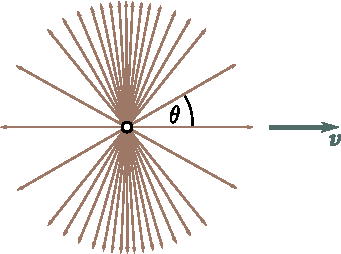
\includegraphics[scale=1]{figures/ch_06/fig_6_2.pdf}
		\caption[]{}
		\label{fig:6_2}
	\end{center}
	\vspace{-0.8cm}
\end{figure}

Khi $v\ll c$, điện trường của điện tích chuyển động tự do tại thời điểm nào đó không quá khác biệt so với điện trường tĩnh sinh ra bởi điện tích đứng yên đặt ở vị trí của điện tích chuyển động vào thời điểm này. Chúng ta nên nhớ rằng điện trường ``tĩnh'' này cũng di chuyển cùng với điện tích. Do đó, điện trường tại mọi điểm trong không gian sẽ thay đổi theo thời gian.

Khi $v$ trở nên đáng kể so với $c$, ta thấy rằng ở khoảng cách cố định với điện tích thì điện trường theo phương vuông góc với $\vec{v}$ mạnh hơn đáng kể so với điện trường theo phương song song với chuyển động (xem \fig{6_2} cho trường hợp $v/c=0.8$). Đường sức điện thưa dần khi tới gần hướng chuyển động và tập trung chủ yếu ở quanh mặt phẳng chứa điện tích và vuông góc với vector $\vec{v}$.

\section{Định luật Biot-Savart}\label{sec:6_4}

Chúng ta sẽ khảo sát từ trường sinh ra bởi một dây mảnh có dòng điện chạy qua. Ta sẽ tập trung vào một đoạn rất nhỏ của dây $\deriv{l}$. Phần tử này chứa $nS\, \deriv{l}$ đường dòng điện ($n$ là số đường dòng trong một đơn vị thể tích, và $S$ là tiết diện của dây ở vị trí của phần tử dây $\deriv{l}$). Xét tại điểm có vị trí tương đối so với phần tử dòng $\deriv{l}$ được xác định bởi vector $\vec{r}$ (\fig{6_3}), một đường dòng $e$ sẽ sinh cảm ứng từ
\begin{equation*}
    \vec{B} = \frac{\mu_0}{4\pi} \frac{e [(\vec{v} + \vec{u}) \times \vec{r}]}{r^3}
\end{equation*}

\noindent
[xem lại \eqn{6_21}]. Ở đây, ta thấy $\vec{v}$ là vận tốc của chuyển động hỗn loạn, còn $\vec{u}$ là vận tốc của chuyển động có trật tự của đường dòng.

\begin{figure}[t]
	\begin{center}
		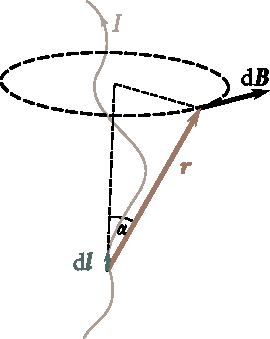
\includegraphics[scale=1]{figures/ch_06/fig_6_3.pdf}
		\caption[]{}
		\label{fig:6_3}
	\end{center}
	\vspace{-0.8cm}
\end{figure}

Giá trị trung bình của cảm ứng từ của mỗi đường dòng có trong phần tử dòng $\deriv{l}$ là
\begin{equation*}
    \average{\vec{B}} = \frac{\mu_0}{4\pi} \frac{e [(\average{\vec{v}} + \average{\vec{u}}) \times \vec{r}]}{r^3} = \frac{\mu_0}{4\pi} \frac{e (\average{\vec{u}} \times \vec{r})}{r^3}
\end{equation*}

\noindent
($\average{\vec{v}}=0$). Nhân biểu thức trên với số đường dòng trong một phần tử dây (tương đương với $nS\, \deriv{l}$), chúng ta suy ra được thành phần từ trường sinh ra bởi $\deriv{l}$:
\begin{equation*}
    \deriv{\vec{B}} = \average{\vec{B}} n S\, \deriv{l} = \frac{\mu_0}{4\pi} \frac{S [(ne\average{\vec{u}}) \times \vec{r}]\, \deriv{l}}{r^3}
\end{equation*}

\noindent
(chúng ta đã đưa các đại lượng vô hướng $n$ và $e$ vào trong tích vector). Vì $ne\average{\vec{u}}=\vec{j}$ nên ta có thể viết lại biểu thức như sau
\begin{equation}\label{eq:6_26}
    \deriv{\vec{B}} = \frac{\mu_0}{4\pi} \frac{S (\vecprod{j}{r})\, \deriv{l}}{r^3}.
\end{equation}

Chúng ta thiết lập đại lượng vector $\deriv{\vec{l}}$ dọc theo trục của phần tử dòng, $\deriv{l}$ cùng chiều với chiều của dòng điện. Độ lớn của vector này là $\deriv{l}$. Do chiều của vector $\vec{j}$ vầ $\deriv{\vec{l}}$ trùng nhau, ta có phương trình 
\begin{equation}\label{eq:6_27}
    \vec{j}\, \deriv{l} = j\, \deriv{\vec{l}}.
\end{equation}

\noindent
Thế vào phương trình \eqn{6_26}, ta được
\begin{equation*}
    \deriv{\vec{B}} = \frac{\mu_0}{4\pi} \frac{S j (\deriv{\vec{l}}\times\vec{r})}{r^3}.
\end{equation*}

\noindent
Cuối cùng, xem xét rằng tích $Sj$ cho ta dòng  $I$ trong dây, ta thu được biểu thức xác định cảm ứng từ sinh ra bởi một phần tử dòng như sau :
\begin{equation}\label{eq:6_28}
    \deriv{\vec{B}} = \frac{\mu_0}{4\pi} \frac{I (\deriv{\vec{l}}\times\vec{r})}{r^3}.
\end{equation}

Ta đã suy ra phương trình \eqn{6_28} từ phương trình \eqn{6_21}. Tuy nhiên, phương trình \eqref{eq:6_28} đã được kiểm chứng bằng thực nghiệm trước khi phương trình \eqn{6_21} được tìm ra . Hơn nữa, phương trình \eqn{6_21} được suy ra từ phương trình \eqn{6_28}.

Vào năm 1820, các nhà Vật Lý người Pháp Jean Biot (1774-1862) và Felix Savart (1791-1841) đã tìm hiểu về từ trường sinh ra chạy trong sợi dây có các hình dạng khác nhau. Nhà thiên văn, nhà toán học Pierre Laplace (1749-1827) phân tích kết quả thực nghiệm thu được và tìm ra rằng từ trường của bất cứ dòng điện nào đều có thể được tính bằng tổng vector ( chồng chập ) của từ trường sinh ra bởi từng phần tử của dòng điện. Laplace thu được phương trình \eqn{6_28} cho cảm ứng từ sinh ra bởi một phần tử dòng có chiều dài $\deriv{l}$.Phương trình  \eqn{6_28} được gọi là   \textbf{ Định luật Biot-Savart-Laplace }, hoặc  \textbf{ Định luật  Biot-Savart}. Hình \fig{6_3} thể hiện rằng vector $\deriv{\vec{B}}$ có hướng vuông góc với mặt phẳng chứa vector $\deriv{\vec{l}}$ và điểm mà từ trường đang được tính sao cho hướng của $\deriv{\vec{l}}$ và hướng quay quanh $\deriv{\vec{l}}$ theo hướng của $\deriv{\vec{B}}$ thoả mãn quy tắc nắm tay phải.
Độ lớn của $\deriv{\vec{B}}$ được xác định bởi biểu thức 
\begin{equation}\label{eq:6_29}
    \deriv{B} = \frac{\mu_0}{4\pi} \frac{I\, \deriv{l}\, \sin\theta}{r^3},
\end{equation}

\noindent
với $\alpha$ là góc hợp bởi vector $\deriv{\vec{l}}$ và vector $\vec{r}$.

Chúng ta sẽ sử dụng \eqn{6_28} để tính từ trường sinh ra bởi dòng điện thẳng, \ie, từ trường sinh ra bởi dòng điện truyền qua dây dẫn thẳng, mảnh và dài vô hạn (\fig{6_4}). Tất cả các vector $\deriv{\vec{B}}$ tại một điểm đều có cùng hướng (trong trường hợp này, hướng của chúng là ngoài hình vẽ). Do đó, thay vì cộng các vector $\deriv{\vec{B}}$ thì ta chỉ cần cộng giá trị của chúng. Chúng ta sẽ tính cảm ứng từ tại điểm cách dây một khoảng là $b$.

\begin{figure}[t]
	\begin{center}
		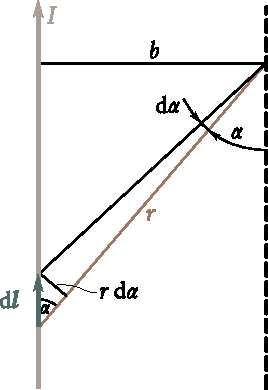
\includegraphics[scale=1]{figures/ch_06/fig_6_4.pdf}
		\caption[]{}
		\label{fig:6_4}
	\end{center}
	\vspace{-0.8cm}
\end{figure}

Xem xét \fig{6_4}, ta có được
\begin{equation*}
    r = \frac{b}{\sin\alpha},\quad \deriv{l} = \frac{r\, \deriv{\alpha}}{\sin\alpha} = \frac{b\, \deriv{\alpha}}{\sin^2\alpha}.
\end{equation*}

\noindent
Thế các giá trị trên vào \eqn{6_29}:
\begin{equation*}
    \deriv{B} = \frac{\mu_0}{4\pi} \frac{Ib\, \deriv{\alpha} \sin\alpha \sin^2\alpha}{b^2 \sin^2\alpha} = \frac{\mu_0}{4\pi} \frac{I}{b} \sin\alpha\, \deriv{\alpha}.
\end{equation*}

Góc $\alpha$ bị giới hạn từ $0$ tới $\pi$ cho mọi phần tử của dòng điện thẳng dài vô hạn. Do đó
\begin{equation*}
    B = \int \deriv{B} = \frac{\mu_0}{4\pi} \frac{I}{b} \int_0^{\pi} \sin\alpha\, \deriv{\alpha} = \frac{\mu_0}{4\pi} \frac{2I}{b}.
\end{equation*}

\noindent
Vậy, cảm ứng từ của dòng điện thẳng có công thức là
\begin{equation}\label{eq:6_30}
    B = \frac{\mu_0}{4\pi} \frac{2I}{b}.
\end{equation}

Các đường sức từ của dòng điện thẳng là các đường tròn đồng tâm quanh dây dẫn (\fig{6_5}).

\begin{figure}[t]
	\begin{center}
		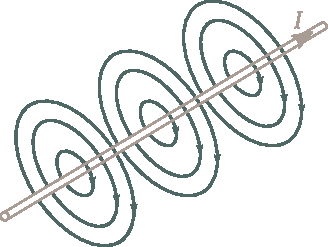
\includegraphics[scale=1]{figures/ch_06/fig_6_5.pdf}
		\caption[]{}
		\label{fig:6_5}
	\end{center}
	\vspace{-0.8cm}
\end{figure}

\section{Lực Lorentz}\label{sec:6_5}

Một điện tích chuyển động trong từ trường sẽ chịu tác dụng của một lực mà ta gọi là \textbf{lực từ}. Lực này phụ thuộc vào điện tích $q$, vận tốc $\vec{v}$, và cảm ứng từ $\vec{B}$ tại vị trí của điện tích vào thời điểm đang xét. Chúng ta có thể giả thiết rằng $F$ tỉ lệ thuận với các đại lượng $q$, $v$, và $B$. Ngoài ra, ta cũng có thể đoán rằng hướng và độ lớn của vector $\vec{F}$ sẽ phụ thuộc vào hướng của các vector $\vec{v}$ và $\vec{B}$. 

Để ``thiết lập'' vector $\vec{F}$ từ đại lượng vô hướng $q$ và các vector $\vec{v}$ và $\vec{B}$, chúng ta sẽ lấy tích vector của $\vec{v}$ và $\vec{B}$ rồi nhân kết quả nhận được với đại lượng vô hướng $q$. Khi đó, ta sẽ thu được biểu thức
\begin{equation}\label{eq:6_31}
    q (\vecprod{v}{B}).
\end{equation}

Thực nghiệm đã cho thấy rằng lực $\vec{F}$ tác dụng lên điện tích chuyển động trong từ trường được biểu diễn bởi công thức
\begin{equation}\label{eq:6_32}
    \vec{F} = k q (\vecprod{v}{B}),
\end{equation}

\noindent
trong đó $k$ là hệ số tỉ lệ phụ thuộc vào hệ đơn vị đang được sử dụng để biểu diễn các đại lượng trong công thức.

Lưu ý rằng không được coi các lập luận được sử dụng để suy ra công thức \eqref{eq:6_31} như cách chứng minh công thức \eqn{6_32}. Các lập luận trên thiếu tính xác thực. Mục đích chính của chúng là để giúp ta nhớ \eqn{6_32}. Công thức trên chỉ có thể được thiết lập bằng thực nghiệm.

Công thức \eqn{6_32} có thể được coi như định nghĩa của cảm ứng từ $\vec{B}$.

Đơn vị của cảm ứng từ $\vec{B}$---tesla----được đặt sao cho hệ số tỉ lệ $k$ trong \eqn{6_32} bằng 1. Do đó, trong hệ đơn vị SI, công thức trên trở thành
\begin{equation}\label{eq:6_33}
    \vec{F} = q (\vecprod{v}{B}).
\end{equation}

Độ lớn của lực từ là
\begin{equation}\label{eq:6_34}
    F = q v B \sin\alpha,
\end{equation}

\noindent
với $\alpha$ là góc hợp bởi vector $\vec{v}$ và vector $\vec{B}$. Ta có thể nhận thấy từ phương trình \eqn{6_34} là một điện tích chuyển động dọc theo đường sức từ sẽ không chịu tác dụng bởi lực từ. 

Lực từ có hướng vuông góc với mặt phẳng chứa vector $\vec{v}$ và vector $\vec{B}$. Nếu điện tích $q$ có dấu dương thì lực từ có hướng trùng với hướng của $vecprod{v}{B}$, còn nếu điện tích $q$ âm thì hướng của lực $\vec{F}$ ngược với hướng của tích $\vecprod{v}{B}$ (\fig{6_6}).

Do hướng của lực từ luôn vuông góc với hướng vận tốc của điện tích chuyển động, lực từ không sinh công lên điện tích. Do đó, ta không thể thay đổi năng lượng của điện tích bằng cách đặt nó trong từ trường đều.

\begin{figure}[t]
	\begin{center}
		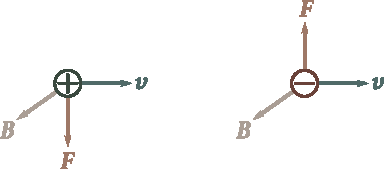
\includegraphics[scale=1]{figures/ch_06/fig_6_6.pdf}
		\caption[]{}
		\label{fig:6_6}
	\end{center}
	\vspace{-0.8cm}
\end{figure}

Lực tác dụng lên một điện tích chuyển động trong đồng thời điện trường và từ trường có biểu thức là
\begin{equation}\label{eq:6_35}
    \vec{F} = q \vec{E} + q (\vecprod{v}{B}).
\end{equation}

\noindent
Biểu thức trên được suy ra từ các kết quả thực nghiệm bởi nhà vật lý người Hà Lan Hendrik Lorentz (1853-1928) và do đó nó được gọi là \textbf{lực Lorentz}.

Giả sử rằng điện tích $q$ đang chuyển động với vận tốc $\vec{v}$ song song với một sợi dây dẫn thẳng dài vô hạn có dòng điện $I$ chạy qua (\fig{6_7}).

Từ \eqns{6_30}{6_34}, hạt mang điện sẽ chịu lực từ có độ lớn là 
\begin{equation}\label{eq:6_36}
    F = qvB = qv \frac{\mu_0}{4\pi} \frac{2I}{b},
\end{equation}

\noindent
trong đó $b$ là khoảng cách từ điện tích tới dây dẫn. Lực sẽ hướng vào dây nếu đây là điện tích dương và chiều của dòng điện và chiều chuyển động của hạt mang điện là như nhau (xem \fig{6_7}). Khi điện tích là âm và các điều kiện khác giữ nguyên, lực sẽ đảo chiều.

Xem xét hai điện tích điểm $q_1$ và $q_2$ di chuyển trên hai đường thẳng song song nhau với cùng vận tốc $v$ nhỏ hơn rất nhiều $c$ (\fig{6_8}). Khi $v\ll c$, điện trường sẽ gần như không đổi so với trường hợp tĩnh (xem \sect{6_3}). Do đó, độ lớn của lực điện $\ab{F}{e}$ tác dụng lên các điện tích sẽ tương đương với
\begin{equation}\label{eq:6_37}
    \ab{F}{e,$1$} = \ab{F}{e,$2$} = \ab{F}{e} = \frac{1}{4\pi\varepsilon_0} \frac{q_1 q_2}{r^2}.
\end{equation}

\begin{figure}[t]
	\begin{minipage}[t]{0.48\linewidth}
		\begin{center}
			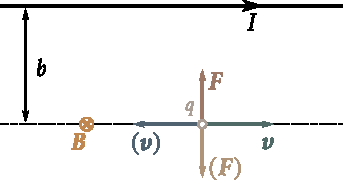
\includegraphics[scale=1]{figures/ch_06/fig_6_7.pdf}
			\caption[]{}
			\label{fig:6_7}
		\end{center}
	\end{minipage}
	\hfill{ }%space{-0.05cm}
	\begin{minipage}[t]{0.48\linewidth}
		\begin{center}
			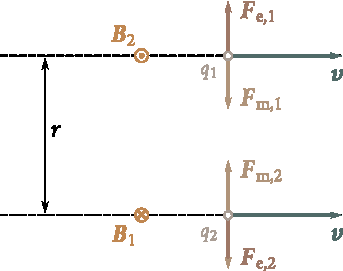
\includegraphics[scale=1]{figures/ch_06/fig_6_8.pdf}
			\caption[]{}
			\label{fig:6_8}
		\end{center}
	\end{minipage}
\vspace{-0.4cm}
\end{figure}

Phương trình \eqref{eq:6_21} và \eqref{eq:6_3} cho ta biểu thức của lực từ tác dụng lên điện tích $\ab{F}{m}$ :
\begin{equation}\label{eq:6_38}
    \ab{F}{m,$1$} = \ab{F}{m,$2$} = \ab{F}{m} = \frac{\mu_0}{4\pi} \frac{q_1 q_2 v^2}{r^2}
\end{equation}

\noindent
( vector toạ độ $\vec{r}$ vuông góc với vector $\vec{v}$).

Chúng ta hãy tìm tỉ số giữa lực điện và lực từ. Từ phương trình \eqns{6_37}{6_38} ta có :  
\begin{equation}\label{eq:6_39}
    \frac{\ab{F}{m}}{\ab{F}{e}} = \varepsilon_0 \mu_0 v^2 = \frac{v^2}{c^2}
\end{equation}

[see \eqn{6_15}].Chúng ta thu được phương trình \eqn{6_39} giả thiết rằng $v\ll c$. Tỉ số này không đổi, với mọi $v$.

Lực điện $\ab{\vec{F}}{e}$ và lực từ $\ab{\vec{F}}{m}$ có hướng ngược nhau. Hình \ref{fig:6_8} đã được vẽ cho 2 điện tích dương giống nhau. Cho 2 điện tích âm giống nhau, hướng của lực tương tác không đổi, còn hướng của từ trường $\vec{B}_1$ và $\vec{B}_2$ bị đảo chiều. Với các điện tích trái dấu, hướng của từ trường và điện trường sẽ đảo ngược lại so với hình vẽ.
Khảo sát phương trình \eqn{6_39} cho ta thấy lực từ yếu hơn lực Coulomb    shows that the magnetic force is weaker than the Coulomb one by a factor equal to the square of the ratio of the speed of the charge to that of light. Lí do cho điều này là tương tác từ giữa các điện tích chuyển động là một hiệu ứng tương đối tính( xem \sect{6_7} ). Từ trường sẽ biến mất nếu vận tốc ánh sáng là vô cùng.

\section{Định luật Ampere}\label{sec:6_6}

Nếu một dây dẫn mang dòng điện được đặt vào trong từ trường thì mỗi phần tử mang điện sẽ chịu lực là
\begin{equation}\label{eq:6_40}
    \vec{F} = e [(\vec{v} + \vec{u}) \times \vec{B}]
\end{equation}

\noindent
[xem lại \eqn{6_33}]. Ở đây, $\vec{v}$ là vận tốc của chuyển động hỗn loạn của hạt mang điện, còn $\vec{u}$ là vận tốc của chuyển động có trật tự. Tác dụng của lực lên hạt mang điện sẽ được truyền đến dây dẫn chứa các hạt này. Hệ quả là xuất hiện một lực tác dụng lên dây dẫn có dòng chạy qua và được đặt trong từ trường.

Chúng ta hãy tìm giá trị của lực $\deriv{\vec{F}}$ tác dụng lên một phần tử dây có chiều dài $\deriv{l}$. Ta lấy giá trị trung bình của \eqn{6_40} trên mọi hạt mang điện trong phần tử dây $\deriv{l}$:
\begin{equation}\label{eq:6_41}
    \average{\vec{F}} = e [(\average{\vec{v}} + \average{\vec{u}}) \times \vec{B}] = e (\average{\vec{u}} \times \vec{B})
\end{equation}

\noindent
($\vec{B}$ là cảm ứng từ tại vị trí của phần từ $\deriv{l}$ ). Phần tử dây chứa $nS\,\deriv{l}$ hạt mang điện ($n$ là số hạt mang điện trên một đơn vị thể tích, còn $S$ là tiết diện của dây tại điểm đang xét). Nhân phương trình \eqn{6_41} với số hạt mang điện, ta tính được lực mà chúng ta đang xem xét :
\begin{equation*}
    \deriv{\vec{F}} = \average{\vec{F}} n S\, \deriv{l} = [(ne\average{\vec{u}}) \times \vec{B}] S\, \deriv{l}.
\end{equation*}

\noindent
 Chú ý rằng $ne\average{\vec{u}}$ là mật độ dòng $\vec{j}$, và $S\,\deriv{l}$ cho ta thể tích của một phần tử dây $\deriv{V}$, ta có
\begin{equation}\label{eq:6_42}
    \deriv{\vec{F}} = (\vecprod{j}{B})\, \deriv{V}.
\end{equation}

\noindent
Từ đó, ta thu được biểu thức của mật độ lực tác dụng lên một đơn vị thể tích của vật dẫn.
\begin{equation}\label{eq:6_43}
    \ab{\vec{F}}{u.v} = \vecprod{j}{B}.
\end{equation}

Viết lại phương trình \eqn{6_42} dưới dạng
\begin{equation*}
    \deriv{\vec{F}} = (\vecprod{j}{B}) S\, \deriv{l}.
\end{equation*}

\noindent
Dựa vào phương trình \eqn{6_27} $\vec{j}S\,\deriv{l}$, ta thay $jS\,\deriv{\vec{l}}= I\,\deriv{\vec{l}}$, ta có phương trình
\begin{equation}\label{eq:6_44}
    \deriv{\vec{F}} = I (\deriv{\vec{l}} \times \vec{B}).
\end{equation}

\noindent
 Phương trình này xác định lực từ tác dụng lên một đơn vị dòng điện   $\deriv{\vec{l}}$ đặt trong từ trường . Phương trình \eqref{eq:6_44} được thiết lập bằng thực nghiệm bởi Ampere và được gọi là \textbf{ Định luật Ampere}.

Chúng ta đã thu được định luật Ampere dựa trên phương trình \eqn{6_33} cho lực từ. Phương trình cho lưc từ trên thực tế được suy ra từ thực nghiệm \eqref{eq:6_44}.

Độ lớn của lực từ \eqref{eq:6_44} được xác định bởi biểu thức
\begin{equation}\label{eq:6_45}
    \deriv{F} = I B\, \deriv{l}\, \sin\alpha,
\end{equation}

\noindent
với góc $\alpha$ là góc hợp giữa vector $\deriv{\vec{l}}$ và vector $\vec{B}$ (\fig{6_9}). Lực có phương pháp tuyến với mặt phẳng chứa vector $\deriv{\vec{l}}$ và $\vec{B}$.

\begin{figure}[t]
	\begin{minipage}[t]{0.35\linewidth}
		\begin{center}
			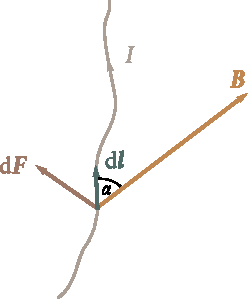
\includegraphics[scale=1]{figures/ch_06/fig_6_9.pdf}
			\caption[]{}
			\label{fig:6_9}
		\end{center}
	\end{minipage}
	\hfill{ }%space{-0.05cm}
	\begin{minipage}[t]{0.59\linewidth}
		\begin{center}
			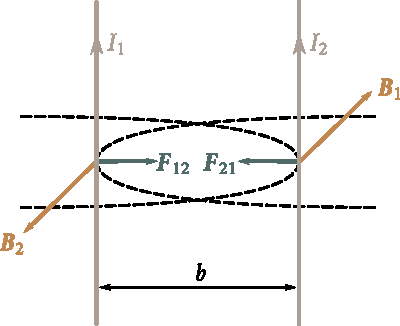
\includegraphics[scale=1]{figures/ch_06/fig_6_10.pdf}
			\caption[]{}
			\label{fig:6_10}
		\end{center}
	\end{minipage}
\vspace{-0.4cm}
\end{figure}

Chúng ta hãy sử dụng định luật Ampere để tính lực tương tác giữa hai dây dẫn thẳng, song song, dài vô hạn có dòng điện chạy qua và được đặt trong chân không. Nếu khoảng cách giữa các dòng điện là $b$ (\fig{6_10}), thì mỗi phần tử của dòng điện $I_2$ sẽ nằm trong từ trường có cảm ứng từ là $B_1=(\mu_0/4\pi)(2I_1/b)$ [xem \eqn{6_30}]. Góc $\alpha$ giữa các phần tử dòng điện $I_2$ và vector $\vec{B}_1$ là góc vuông. Do vậy, từ \eqn{6_45}, lực tác dụng lên một đơn vị độ dài của dòng điện $I_2$ là
\begin{equation}\label{eq:6_46}
    \ab{F}{21,u} = I_2 B_1 = \frac{\mu_0}{4\pi} \frac{2 I_1 I_2}{b}.
\end{equation}

\noindent
Biểu thức \eqref{eq:6_46} khớp với \eqn{6_2}.

Chúng ta sẽ có công thức tương tự cho lực $\ab{F}{21,u}$ tác dụng lên một đơn vị độ dài của dòng $I_1$. Dễ thấy rằng khi dòng chạy theo cùng hướng, chúng sẽ hút nhau và khi dòng chạy ngược chiều nhau, chúng sẽ đẩy nhau.

\section{Từ trường dưới góc nhìn Tương đối tính}\label{sec:6_7}

Điện và từ có mối liên hệ rất chặt chẽ. Dựa trên các tiên đề của thuyết tương đối và sự bất biến của điện tích, ta có thể cho thấy rằng tương tác từ giữa các điện tích và dòng điện là hệ quả của định luật Coulomb. Chúng ta sẽ sử dụng ví dụ của một điện tích chuyển động với vận tốc $v_0$\footnote{Chúng ta kí hiệu vận tốc của điện tích là $v_0$ để giống với kí hiệu được sử dụng trong Chương 8 của Vol. I.} song song với dòng điện thẳng dài vô hạn để cho thấy nhận định trên (\fig{6_11}).

Theo \eqn{6_36}, lực từ tác dụng lên điện tích trong trường hợp đang xét đến là
\begin{equation}\label{eq:6_47}
    F = q v_0 \frac{\mu_0}{4\pi} \frac{2 I}{b}
\end{equation}

\noindent
(ý nghĩa của các kí hiệu được giải thích trong \fig{6_11}). Lực trên hướng vào dây dẫn mang dòng điện ($q>0$). Trước khi ta bắt đầu chứng minh \eqn{6_47} dựa trên định luật Coulomb và các liên hệ tương đối tính, hãy xem xét hiệu ứng sau. Giả thiết ta có một chuỗi các điện tích có độ lớn như nhau là $e$ đặt cách nhau một khoảng rất nhỏ $l_0$ (\fig{6_12}). Do $l_0$ rất nhỏ, chúng ta có thể tính ra mật độ điện dài $\lambda_0$:
\begin{equation}\label{eq:6_48}
    \lambda_0 = \frac{e}{l_0}.
\end{equation}

\begin{figure}[t]
	\begin{minipage}[t]{0.48\linewidth}
		\begin{center}
			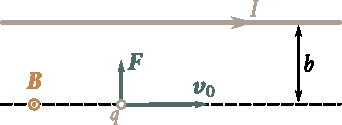
\includegraphics[scale=1]{figures/ch_06/fig_6_11.pdf}
			\caption[]{}
			\label{fig:6_11}
		\end{center}
	\end{minipage}
	\hfill{ }%space{-0.05cm}
	\begin{minipage}[t]{0.48\linewidth}
		\begin{center}
			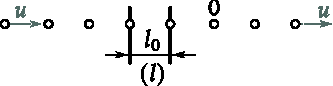
\includegraphics[scale=1]{figures/ch_06/fig_6_12.pdf}
			\caption[]{}
			\label{fig:6_12}
		\end{center}
	\end{minipage}
\vspace{-0.4cm}
\end{figure}

\noindent
Chúng ta sẽ cho các điện tích trên chuỗi chuyển động dọc theo chuỗi với vận tốc như nhau $u$. Khoảng cách giữa các điện tích sẽ giảm và bằng
\begin{equation*}
    l = l_0 \bracket{1 - \frac{u^2}{c^2}}^{1/2}
\end{equation*}

\noindent
[xem Eq. 8.19 của Vol. I]. Do giá trị độ lớn của điện tích là hằng số, nên mật độ điện tích dài trong hệ quy chiếu gắn với các điện tích đang chuyển động sẽ thay đổi và trở thành 
\begin{equation}\label{eq:6_49}
    \lambda = \frac{e}{l} = \frac{\lambda_0}{\sqrt{1 - \parenthesis{u^2/v^2}}}.
\end{equation}

Giờ chúng ta xét trong hệ quy chiếu K, hai dòng điện tích có cùng độ lớn, nhưng ngược dấu, chuyển động ngược nhau với vận tốc $u$  và xấp xỉ trùng nhau (\fig{6_13}a) . Sự kết hợp của 2 dòng điện tích này tương đương một dòng điện dài vô hạn có giá trị là. 
\begin{equation}\label{eq:6_50}
    I = 2 \lambda u = \frac{2 \lambda_0 u}{\sqrt{1 - \parenthesis{u^2/v^2}}},
\end{equation}

\noindent
 với  $\lambda$ là đại lượng được xác định bởi phương trình \eqn{6_49}. Tông mật độ điện  dài của dòng điện tích bằng 0, nên không xuất hiện điện trường. Điện tích $q$ chịu lực từ có độ lớn được tính từ phương trình \eqns{6_47}{6_50} có giá trị là
\begin{equation}\label{eq:6_51}
    F = q v_0 \frac{\mu_0}{4\pi} \frac{4 \lambda_0 u}{b \sqrt{1 - \parenthesis{u^2/v^2}}}.
\end{equation}

\begin{figure}[t]
	\begin{center}
		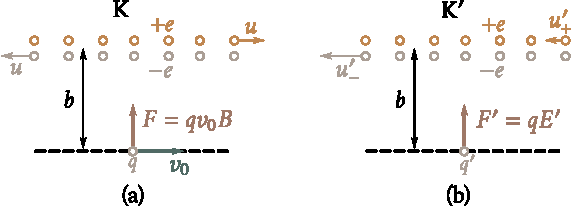
\includegraphics[scale=1]{figures/ch_06/fig_6_13.pdf}
		\caption[]{}
		\label{fig:6_13}
	\end{center}
	\vspace{-0.8cm}
\end{figure}

Giờ chúng ta xem xét trong hệ quy chiếu K$'$ khi mà điện tích $q$ đứng yên. (\fig{6_13}b). Trong hệ quy chiếu này, điện tích $q$ cũng chịu lực ( kí hiệu là $F'$ ). Lực này không phải là lực từ, do điện tích $q$ đang đứng yên. Lực $F'$ thuần tuý là lực điện. Trong trường hợp này lực điện xuất hiện do mật độ điện tích dài của dòng điện tích dương và dòng điện tích âm là khác nhau ( ta sẽ thấy ở dưới là dòng điện tích âm có giá trị lớn hơn ). Sự chênh lệch mật độ điện tích ở hai dòng điện tích sinh ra điện trường tác dụng lực $F’$ lên điện tích dương $q$ hướng về phía dòng điện tích (xem hình  \fig{6_13}b).

GIờ ta xem xét lực $F’$ để thuyết phục chúng ta rằng là nó “bằng” với lực $F$ tính bởi phương trình \eqn{6_51}. Từ "bằng" được đặt trong dấu ngoặc kép vì lực không phải một đại lượng bất biến. Khi chuyển từ một hệ quy chiếu quán tính này sang một hệ quy chiếu quán tính khác, lực được biến đổi theo một định luật khá là phức tạp. Trong trường hợp cụ thể này, khi mà lực $\vec{F}'$ vuông góc với vận tốc tương đối giữa hệ quy chiếu K và K’, ($\vec{F}' \perp \vec{v}_0$), phép biến đổi có dạng
\begin{equation*}
    \vec{F} = \frac{\vec{F}' \sqrt{1 - \parenthesis{v_0^2/c^2}} + \vec{v}_0 (\vec{F}'\ccdot\vec{v}')/c^2}{1 + (\vec{v}_0\ccdot\vec{v}')/c^2}
\end{equation*}

\noindent
($\vec{v}'$ là vận tốc của một hạt chiu lực $\vec{F}'$ trong hệ quy chiếu K'). Nếu $\vec{v}'=0$ ( trong trường hợp này ta đang xét ), công thức cho sự biến đổi của lực có dạng như sau:
\begin{equation*}
    \vec{F} = \vec{F}' \bracket{1 - \parenthesis{ \frac{v_0^2}{c^2} }}^{1/2}.
\end{equation*}

Từ phương trình này, ta thấy lực vuông góc với $\vec{v}_0$ tác dụng lên điện tích ở trạng thái nghỉ trong hệ quy chiếu K' cũng vuông góc với vector $\vec{v}_0$ trong hệ quy chiéu K. Độ lớn của lực trong trường hợp này, được tính bởi công thức :
\begin{equation}\label{eq:6_52}
    F = F' \bracket{1 - \parenthesis{ \frac{v_0^2}{c^2} }}^{1/2}.
\end{equation}

Mật độ điện tích dài của dòng điện tích dương và dòng điện tích âm trong hệ quy chiếu K' có giá trị là [ xem phương trình  \eqn{6_49}]
\begin{equation}\label{eq:6_53}
    \lambda_+' = \frac{\lambda_0}{\sqrt{1 - \parenthesis{u_+'^2/c^2}}},\quad \lambda_-' = - \frac{\lambda_0}{\sqrt{1 - \parenthesis{u_-'^2/c^2}}},
\end{equation}

\noindent
với $u_+'$ và $u_-'$ là vận tốc của điện tích $+e$ và $-e$ trong hệ quy chiếu K'. Chuyển từ hệ quy chiêu K sang hệ quy chiếu K', hình chiếu của vận tốc của hạt lên trục $x$ trùng với hướng của $\vec{v}_0$ được biến đổi theo phương trình
\begin{equation*}
    u_x' = \frac{u_x - v_0}{1 - \parenthesis{u_xv_0/c^2}}
\end{equation*}

\noindent
[ xem phương trình (8.28) của Vol. I; ta thế $u$ và $u'$ cho $v$ và $v'$]. Cho điện tích $+e$, thành phần $u_x$ bằng $u$, với $-e$ thì bằng $-u$ ( xem hình \fig{6_13}a). Do đó,
\begin{equation*}
    \parenthesis{u_x'}_+ = \frac{u - v_0}{1 - \parenthesis{uv_0/c^2}},\quad \parenthesis{u_x'}_- = \frac{-u - v_0}{1 + \parenthesis{uv_0/c^2}}.
\end{equation*}

\noindent
Do thành phần vận tốc theo các phương còn lại bằng 0, ta có
\begin{equation}\label{eq:6_54}
    u_+' = \frac{|u - v_0|}{1 - \parenthesis{uv_0/c^2}},\quad u_-' = \frac{u + v_0}{1 + \parenthesis{uv_0/c^2}}.
\end{equation}

Để đơn giản hoá các phép toán, chúng ta dùng các biến không thứ nguyên sau ( chia các vận tốc cho $c$ ):
\begin{equation*}
    \beta_0 = \frac{v_0}{c},\quad \beta = \frac{u}{c},\quad \beta_+' = \frac{u_+'}{c},\quad \beta_- = \frac{u_-'}{c}.
\end{equation*}

\noindent
Phương trình \eqref{eq:6_53} và \eqref{eq:6_54} từ đó có dạng
\begin{align}
    \lambda_+' &= \frac{\lambda_0}{\sqrt{1 - \beta_+'^2}},\quad \lambda_- = \frac{\lambda_0}{\sqrt{1 - \beta_-'^2}} \label{eq:6_55}\\
    \beta_+' &= \frac{|\beta - \beta_0|}{1 - \beta \beta_0},\quad \beta_-' = \frac{\beta + \beta_0}{1 + \beta \beta_0}.
\end{align}

\noindent 
Dựa trên các phương trình ta đã thu được, ta có biểu thức cho tổng mật độ điện tích dài của hệ:
\begin{align*}
    \lambda' &= \lambda_+' + \lambda_-'\\
    &= \frac{\lambda_0}{\bracket{ 1 - \parenthesis{ \dfrac{\beta-\beta_0}{1-\beta\beta_0} }^2}^{1/2}} - \frac{\lambda_0}{\bracket{ 1 - \parenthesis{ \dfrac{\beta+\beta_0}{1+\beta\beta_0} }^2}^{1/2}}\\
    &= \frac{\lambda_0 \parenthesis{1-\beta\beta_0}}{\sqrt{\parenthesis{1-\beta\beta_0}^2 - \parenthesis{\beta-\beta_0}^2}} - \frac{\lambda_0 \parenthesis{1+\beta\beta_0}}{\sqrt{\parenthesis{1+\beta\beta_0}^2 - \parenthesis{\beta+\beta_0}^2}}.
\end{align*}

\noindent
Dễ dàng nhận thấy 
\begin{equation*}
    \parenthesis{1-\beta\beta_0}^2 - \parenthesis{\beta-\beta_0}^2 = \parenthesis{1+\beta\beta_0}^2 - \parenthesis{\beta+\beta_0}^2 = \parenthesis{1-\beta_0^2} \parenthesis{1+\beta^2}.
\end{equation*}

\noindent
Từ đó,
\begin{equation}\label{eq:6_57}
    \lambda' = \frac{-2 \lambda_0 \beta \beta_0}{\sqrt{\parenthesis{1-\beta_0^2} \parenthesis{1+\beta^2}}} = \frac{-2 \lambda_0 u v_0}{c^2 \sqrt{1 - \parenthesis{v_0^2/c^2}} \sqrt{1 - \parenthesis{u^2/c^2}}}.
\end{equation}

Từ \eqn{1_122}, ta có được điện trường sinh ra bởi dây thẳng, dài vô hạn và có mật độ điện dài $\lambda'$ tại điểm cách dây một khoảng $b$ là
\begin{equation*}
    E' = \frac{1}{2\pi\varepsilon_0} \frac{\lambda'}{b}.
\end{equation*}

\noindent
Trong trường trên, lực tác dụng lên điện tích $q$ là 
\begin{equation*}
    F' = q E' = \frac{q \lambda'}{2\pi\varepsilon_0 b}.
\end{equation*}

\noindent
Thay \eqn{6_57} vào, ta được (ở đây chúng ta đã bỏ dấu trừ đi)
\begin{align}
    F' &= \frac{q\lambda_0 u v_0}{ \pi\varepsilon_0 vc^2 \sqrt{1 - \parenthesis{v_0^2/c^2}} \sqrt{1 - \parenthesis{u^2/c^2}} } \nonumber\\
    &= qv_0 \frac{\mu_0}{4\pi} \frac{4\lambda_0 u}{\sqrt{1 - \parenthesis{u^2/c^2}}} \frac{1}{\sqrt{1 - \parenthesis{v_0^2/c^2}}} \label{eq:6_58}
\end{align}

\noindent
[lưu ý rằng $\mu_0=1/(\varepsilon_0c^2)$; xem lại \eqn{6_15}].

Biểu thức trên chỉ khác \eqn{6_51} một hằng số nhân $\sqrt{1 - \parenthesis{v_0^2/c^2}}$. Do đó, ta có thể viết
\begin{equation*}
    F = F' \bracket{ 1 - \parenthesis{\frac{v_0^2}{c^2}} }^{1/2},
\end{equation*}

\noindent
trong đó $F$ là lực được tính ra từ \eqn{6_51}, còn $F'$ là lực được tính ra từ \eqn{6_58}. So sánh với \eqn{6_52}, ta thấy được $F$ và $F'$ là các giá trị của cùng một lực nhưng ở hai hệ quy chiếu khác nhau K và K'.

Chú ý rằng trong hệ quy chiếu $K'$ chuyển động với vận tốc khác $v_0$ so với hệ quy chiều K, lực tác dụng lên điện tích sẽ bao gồm cả lực điện và lực từ.

Các kết quả ta thu được cho thấy điện trường và từ trường có mối liên hệ mật thiết với nhau và tạo thành một trường điện từ thống nhất. Với những hệ quy chiếu đặc biệt, có thể chỉ còn thành phần điện trường hoặc từ trường. Tuy vậy, với các hệ quy chiếu khác, ta sẽ thấy sự xuất hiện của cả điện trường và từ trường.

Trong các hệ quy chiếu quán tính khác nhau, điện trường và từ trường sinh ra bởi một tập hợp các điện tích sẽ khác nhau. Các phương trình miêu tả sự biến đổi của điện từ trường khi chuyển từ hệ quy chiếu K sang hệ quy chiếu K' di chuyển với vận tốc $\vec{v}_0$ tương đối so với K (cách chứng minh cho hệ thức biến đổi trên vượt quá chương trình của cuốn sách này) là
\begin{equation}\label{eq:6_59}
    \begin{cases}
        & \!\!\!\!\! E_x' = E_x,\quad E_y = \dfrac{E_y-v_0B_z}{\sqrt{1-\beta^2}},\quad E_z' = \dfrac{E_z+v_0B_y}{\sqrt{1-\beta^2}},\\
        & \!\!\!\!\! B_x' = B_x,\quad B_y = \dfrac{B_y+v_0E_z}{\sqrt{1-\beta^2}},\quad B_z' = \dfrac{B_z-v_0E_y}{\sqrt{1-\beta^2}}.
    \end{cases}
\end{equation}

Ở đây, $E_x$, $E_y$, $E_z$, $B_x$, $B_y$, $B_z$ là các thành phần của các vector $\vec{E}$ và $\vec{B}$ đặc trưng cho trường điện từ trong hệ quy chiếu K, còn các biểu tượng $E_x'$, $E_y'$, $E_z'$, $B_x'$, $B_y'$, $B_z'$ là các thành phần tương ứng của các vector $\vec{E}'$ và $\vec{B}'$ đặc trưng cho trường trong hệ quy chiếu K'. Kí tự Hy Lạp $\beta$ được dùng để kí hiệu tỉ số $v_0/c$.

Nếu ta tách các vector $\vec{E}$ và $\vec{B}$ cũng như $\vec{E}'$ và $\vec{B}'$ thành các thành phần song song với vector $\vec{v}_0$ (và cũng là thành phần hướng theo trục $x$ và $x'$) và thành phần vuông góc với vector này (\ie, chẳng hạn, ta có thể biểu diễn $\vec{E}$ dưới dạng $\vec{E}=\vec{E}_{\parallel}+\vec{E}_{\perp}$, etc.), ta có thể viết lai Eqs. \eqref{eq:6_59} dưới dạng vector:
\begin{equation}\label{eq:6_60}
    \begin{cases}
        & \!\!\!\!\! \vec{E}_{\parallel}' = \vec{E}_{\parallel},\quad \vec{E}_{\perp}' = \dfrac{\vec{E}_{\perp} + (\vec{v}_0 \times \vec{B}_{\perp})}{\sqrt{1-\beta^2}},\\
        & \!\!\!\!\! \vec{B}_{\parallel}' = \vec{B}_{\parallel},\quad \vec{B}_{\perp}' = \dfrac{\vec{B}_{\perp}- \parenthesis{1/c^2} (\vec{v}_0 \times \vec{E}_{\perp})}{\sqrt{1-\beta^2}}.
    \end{cases}
\end{equation}

\noindent
Trong hệ đơn vị Gauss, hệ thức \eqref{eq:6_60} có dạng là
\begin{equation}\label{eq:6_61}
    \begin{cases}
        & \!\!\!\!\! \vec{E}_{\parallel}' = \vec{E}_{\parallel},\quad \vec{E}_{\perp}' = \dfrac{\vec{E}_{\perp} + \parenthesis{1/c} (\vec{v}_0 \times \vec{B}_{\perp})}{\sqrt{1-\beta^2}},\\
        & \!\!\!\!\! \vec{B}_{\parallel}' = \vec{B}_{\parallel},\quad \vec{B}_{\perp}' = \dfrac{\vec{B}_{\perp}- \parenthesis{1/c} (\vec{v}_0 \times \vec{E}_{\perp})}{\sqrt{1-\beta^2}}.
    \end{cases}
\end{equation}

\noindent
Khi $\beta\ll 1$ (\ie, $v_0\ll c$), biểu thức \eqref{eq:6_60} được đơn giản hóa:
\begin{align*}
    \vec{E}_{\parallel}' &= \vec{E}_{\parallel},\quad \vec{E}_{\perp}' = \vec{E}_{\perp} + \vec{v}_0 \times \vec{B}_{\perp},\\
    \vec{B}_{\parallel}' &= \vec{B}_{\parallel},\quad \vec{B}_{\perp}' = \vec{B}_{\perp}-\parenthesis{1/c^2} (\vec{v}_0 \times \vec{E}_{\perp}).
\end{align*}

\noindent
Cộng các phương trình trên vào nhau, ta được
\begin{equation}\label{eq:6_62}
    \begin{cases}
        & \!\!\!\!\! \vec{E}' = \vec{E}_{\parallel}' + \vec{E}_{\perp}' = \vec{E}_{\parallel} + \vec{E}_{\perp} + (\vec{v}_0 \times \vec{B}_{\perp}) = \vec{E} + (\vec{v}_0 \times \vec{B}_{\perp}),\\
        & \!\!\!\!\! \vec{B}' = \vec{B}_{\parallel}' + \vec{B}_{\perp}' = \vec{B}_{\parallel} + \vec{B}_{\perp} - \dfrac{1}{c^2} (\vec{v}_0 \times \vec{E}_{\perp}) = \vec{B} + \dfrac{1}{c^2} (\vec{v}_0 \times \vec{E}_{\perp}).
    \end{cases}
\end{equation}

Do các vector $\vec{v}_0$ và $\vec{B}_{\parallel}$ cùng phương nên tích vector của chúng bằng không. Vì vậy mà $\vec{v}_0 \times \vec{B} = \vec{v}_0 \times \vec{B}_{\parallel} + \vec{v}_0 \times \vec{B}_{\perp} = \vec{v}_0 \times \vec{B}_{\perp}$.
Tương tự, $\vec{v}_0 \times \vec{E} = \vec{v}_0 \times \vec{E}_{\perp}$. Từ đây, ta có thể viết lại hệ thức \eqref{eq:6_62} như sau
\begin{equation}\label{eq:6_63}
    \vec{E}' = \vec{E} + \vec{v}_0 \times \vec{B},\quad \vec{B}' = \vec{B} - \dfrac{1}{c^2} (\vec{v}_0 \times \vec{E}).
\end{equation}

\noindent
Các trường sẽ biến đổi như trên nếu vận tốc tương đối $v_0$ của hệ quy chiếu K' nhỏ hơn rất nhiều vận tốc ánh sáng trong chân không $c$ ($v_0\ll c$).

Các phương trình \eqref{eq:6_63} sẽ có dạng sau nếu được biểu diễn bằng hệ đơn vị Gauss:
\begin{equation}\label{eq:6_64}
    \vec{E}' = \vec{E} + \dfrac{1}{c} (\vec{v}_0 \times \vec{B}),\quad \vec{B}' = \vec{B} - \dfrac{1}{c} (\vec{v}_0 \times \vec{E}).
\end{equation}

Ở ví dụ xét trong hệ quy chiếu K lúc mở đầu phần, trong đó ta có điện tích $q$  di chuyển với vận tốc $\vec{v}_0$ song song với dây dẫn mang dòng điện, chỉ xuất hiện thành phần $\vec{B}_{\perp}$ vuông góc với $\vec{v}_0$; các thành phần $\vec{B}_{\parallel}$, $\vec{E}_{\perp}$. và $\vec{E}_{\parallel}$ bằng không.
Từ hệ thức \eqref{eq:6_60} trong hệ quy chiếu K', trong đó điện tích $q$ đứng yên (hệ quy chiếu này chuyển động với vận tốc $\vec{v}_0$ tương đối so với K), thành phần $\vec{B}_{\perp}'$ bằng với $\vec{B}_{\perp}/\sqrt{1-\beta^2}$ và xuất hiện thêm thành phần vuông góc của điện trường là $\vec{E}_{\perp}'=(\vec{v}_0 \times \vec{B}_{\perp})/\sqrt{1-\beta^2}$.

Trong hệ quy chiếu K, điện tích chịu tác dụng của lực 
\begin{equation}\label{eq:6_65}
    \vec{F} = q (\vec{v}_0 \times \vec{B}_{\perp}).
\end{equation}

\noindent
Do điện tích $q$ không chuyển động trong hệ quy chiếu K', sẽ chỉ có lực điện tác dụng lên nó trong hệ quy chiếu này
\begin{equation}\label{eq:6_66}
    \vec{F}' = q \vec{E}_{\perp}' = \frac{q (\vec{v}_0 \times \vec{B}_{\perp})}{\sqrt{1-\beta^2}}.
\end{equation}

\noindent
Từ \eqns{6_65}{6_66}, ta được kết quả là $\vec{F} = \vec{F}' \sqrt{1-\beta^2}$, giống với kết quả có được từ \eqn{6_52}.

l\section{ Dòng điện kín đặt trong từ trường }\label{sec:6_8}

Ta sẽ khảo sát các tính chất của 1 vòng dây kín mang dòng điện khi đặt trong từ trường, bắt đầu với giả thiết từ trường đều  ($\vec{B}=\text{constant}$). Từ phương trình \eqn{6_44}, một phần tử của vòng dây $\deriv{\vec{l}}$ chịu lực 
\begin{equation}\label{eq:6_67}
    \deriv{\vec{F}} = I (\upd\vecprod{l}{B}).
\end{equation}

\noindent
Tổng hơp của các lực tác dụng lên từng phần tử của vòng dây là \begin{equation}\label{eq:6_68}
    \vec{F} = \oint I (\upd\vecprod{l}{B}).
\end{equation}

\noindent
 Đưa các hằng số  $I$ và $\vec{B}$ ra ngoài tích phân, ta có
\begin{equation*}
    \vec{F} = I \bracket{ \parenthesis{\oint \deriv{\vec{l}} } \times \vec{B} }.
\end{equation*}

\noindent
 Tích phân $\oint\deriv{\vec{l}}$ bằng 0, do đó, $\vec{F}=0$. Vì thế, tổng hợp lực tác dụng lên một dòng điện kín đặt trong từ trường đều bằng 0. Điều này đúng cho mọi đường kín với hình dạng bất kì ( bao gồm các đường cong không đồng phẳng ) và với tất cả các cách sắp xếp của đường kín này trong từ trường. Chỉ có tính đồng nhất của từ trường là cần thiết để cho tổng hợp lực bằng 0.

Trong phần kế tiếp, ta sẽ chi xét đến các đường cong đồng phẳng. Xét tổng hợp moment lực sinh ra bởi các lực tác dung lên đường kín. Do tổng của các lực tác dụng lên đường kín bằng 0 trong từ trường đều, tổng hợp moment lực xét với bất kì trục quay nào cũng như nhau. Thật vậy, tổng hợp moment lực so với trục quay qua điểm $0$ được xác định bởi biểu thức
\begin{equation*}
    \vec{T} = \int (\vec{r} \times \deriv{\vec{F}}),
\end{equation*}

\noindent
với $\vec{r}$ là vector vị trí từ điểm $0$ đến điểm đặt lực $\deriv{\vec{F}}$. Xét điểm $0'$ lệch so với điểm $0$ một đoạn $b$. Do đó, $\vec{r}=\vec{b}+\vec{r}'$ hay $\vec{r}'=\vec{r}-\vec{b}$. Từ đó, tổng hợp moment lực so với trục quay qua điểm $0'$ là 
\begin{align*}
    \vec{T}' &=  \int (\vec{r}' \times \deriv{\vec{F}}) = \int ([\vec{r} - \vec{b}] \times \deriv{\vec{F}}) = \int (\vec{r} \times \deriv{\vec{F}}) - \int (\vec{b} \times \deriv{\vec{F}})\\
    &= \vec{T} - \bracket{ \vec{b} \times \int \deriv{\vec{F}} } = \vec{T},
\end{align*}

\noindent
$\int\deriv{\vec{F}}=0$. Tổng hợp moment lực tính được so với hai trục quay bất kì $0$ và $0'$ là trùng nhau. Do đó, ta kết luận rằng tổng hợp moment lực lên vòng dây không phụ thuộc vào vị trí của trục quay ( giống với ngẫu lực ) 
\begin{figure}[t]
	\begin{center}
		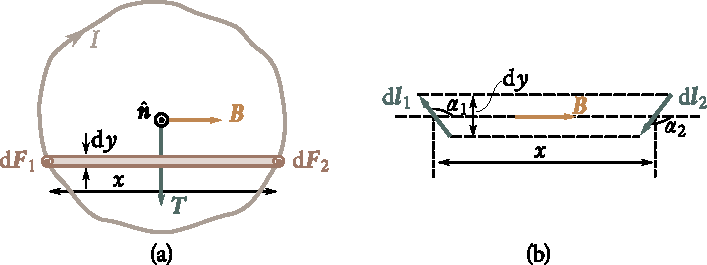
\includegraphics[scale=1]{figures/ch_06/fig_6_14.pdf}
		\caption[]{}
		\label{fig:6_14}
	\end{center}
	\vspace{-0.8cm}
\end{figure}

Xem xét một dòng kín đồng phẳng bất kì đặt trong từ trường đều $\vec{B}$. Giả sử dòng kín được đặt sao cho vector pháp tuyến $\hatvec{n}$ của nó có chiều dương vuông góc với vector $\vec{B}$. (\fig{6_14}). Vector pháp tuyến có chiều dương trùng với chiều dương của vector dòng điện xác định bởi quy tắc nắm tay phải.

Chia diện tích bao bởi dòng kín thành các dải mảnh có chiều dày $\deriv{y}$ song song với chiều của vector $\vec{B}$ ( xem hình \fig{6_14}a; hình \fig{6_14}b là bản phóng to của một dải được nêu ). Lực $\deriv{\vec{F}}_1$ hướng vào hình vẽ được tác dụng vào một phần tử $\deriv{\vec{l}}_1$   bao phía bên trái của dải vừa được cắt ra. Độ lớn của lực này là $\deriv{F}_1 = IB\, \deriv{l}_1\, \sin\alpha_1 = IB\, \deriv{y}$ ( xem hình \fig{6_14}b).
Lực  $\deriv{\vec{F}}_2$ tác dụng hướng ra khỏi mặt phẳng được tác dụng vào phần tử dây $\deriv{\vec{l}}_2$ bao phía bên phải của dải. Độ lớn của lực này là  $\deriv{F}_2 = IB\, \deriv{l}_2\, \sin\alpha_2 = IB\, \deriv{y}$.

Kết quả mà ta thu được chứng tỏ rằng lực tác dụng lên 2 phần tử vòng dây đối xứng nhau $\deriv{\vec{l}}_1$ và $\deriv{\vec{l}}_2$ sinh ra moment lực có biểu thức là
\begin{equation*}
    \deriv{T} = I B x\, \deriv{y} = I B\, \deriv{S}
\end{equation*}

\noindent
($\deriv{S}$  là diện tích của dải ). Phương trình  \fig{6_14} cho thấy vector  $\deriv{\vec{T}}$ có phương vuông góc với vector $\hatvec{n}$ và vector $\vec{B}$ và do đó có thể viết lại dưới dạng
\begin{equation*}
    \deriv{\vec{T}} = I (\hatvec{n} \times \vec{B})\, \deriv{S}.
\end{equation*}

\noindent
Xét tổng của các moment của các dải trên cả vòng dây cho ta tổng hợp moment lực tác dụng lên cả vòng dây :
\begin{equation}\label{eq:6_69}
    \vec{T} = \int I (\hatvec{n} \times \vec{B})\, \deriv{S} = I (\hatvec{n} \times \vec{B}) \int \deriv{S} = I (\hatvec{n} \times \vec{B})\, \deriv{S}
\end{equation}

\noindent
(Từ trường đang được giả thiết là từ trường đồng nhất, do đó tích  $\hatvec{n}\times\vec{B}$ là như nhau cho mọi dải mảnh và có thể được đặt ngoài dấu tích phân.)   Đại lượng $S$ trong phương trình \eqn{6_69} là diện tích của cả vòng dây.

Phương trình \eqref{eq:6_69} có thể được viết dưới dạng
\begin{equation}\label{eq:6_70}
    \vec{T} = (I S \hatvec{n}) \times \vec{B}.
\end{equation}

\noindent
Phương trình này giống như phương trình \eqn{6_58} khi xác định moment lực tác dụng lên lưỡng cực điện đặt trong điện trường. Tương đương với vector $\vec{E}$ trong phương trình \eqn{6_70} là vector $\vec{B}$, còn với moment lượng cực điện $\vec{p}$ là biểu thức $IS\hatvec{n}$. Đây là nguyên nhân gọi đại lượng
\begin{equation}\label{eq:6_71}
    \ab{\vec{p}}{m} = I S \hatvec{n}
\end{equation}

\noindent
 là  \textbf{ moment lưỡng cực từ} của một dòng điện kín. Hướng của vector $\ab{\vec{p}}{m}$  trùng với chiều dương của vector pháp tuyến của vòng dây. 
Dùng các kí hiệu của phương trình \eqn{6_71}, ta có thể viết phương trình \eqn{6_70} như sau:
\begin{equation}\label{eq:6_72}
    \vec{T} = \ab{\vec{p}}{m} \times \vec{B}\quad (\ab{\vec{p}}{m} \perp \vec{B}).
\end{equation}

\begin{figure}[t]
	\begin{center}
		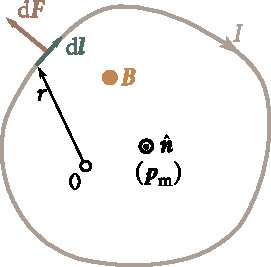
\includegraphics[scale=1]{figures/ch_06/fig_6_15.pdf}
		\caption[]{}
		\label{fig:6_15}
	\end{center}
	\vspace{-0.8cm}
\end{figure}

Giờ, chúng ta sẽ giả thiết rằng $\vec{B}$ cùng hướng với vector pháp tuyến của vòng $\hatvec{n}$ và, do đó, cũng cùng hướng với cả vector $\ab{\vec{p}}{m}$ (\fig{6_15}). Trong trường hợp này, lực tác dụng lên các phần khác nhau của vòng đều nằm trong một mặt phẳng---mặt phẳng vòng dây. Lực tác dụng lên một phần tử dây $\deriv{\vec{l}}$ được tính từ \eqn{6_67}. Chúng ta sẽ tính moment lực tổng hợp quanh điểm $0$ trong mặt phẳng vòng dây được sinh ra từ các lực trên:
\begin{equation*}
    \vec{T} = \int \deriv{\vec{T}} = \int (\vec{r} \times \deriv{\vec{F}}) = I \oint [\vec{r} \times (\deriv{\vec{l}} \times \vec{B})]
\end{equation*}

\noindent
($\vec{r}$ là vector vị trí được nối từ điểm $0$ đến phần tử dây $\deriv{\vec{l}}$). Ta có thể sử dụng Eq. (1.35) từ Vol. I để biến đổi tích phân trên. Hệ quả là
\begin{equation*}
    \vec{T} = I \bracket{ \oint (\vecdot{r}{B})\, \deriv{\vec{l}} - \oint \vec{B} (\vec{r} \ccdot \deriv{\vec{l}}) }.
\end{equation*}

Tích phân đầu tiên bằng không do $\vec{r}$ và $\vec{B}$ vuông góc nhau. Đại lượng vô hướng xuất hiện trong tích phân thứ hai là $r\,\deriv{r} = \deriv{\parenthesis{r^2}}/2$. Do vậy, tích phân thứ hai có thể được viết lại như sau
\begin{equation*}
    \frac{1}{2} \vec{B} \oint \deriv{\parenthesis{r^2}}.
\end{equation*}

\noindent
Vi phân toàn phần của $r^2$ nằm trong tích phân mà tích phân của một hàm trên một đường kín bằng không. Do đó, thành phần thứ hai trong biểu thức của $\vec{T}$ cũng bằng không. Vậy, chúng ta đã chứng minh được rằng moment lực $\vec{T}$ quanh điểm $0$ bất kì trong mặt phẳng của vòng dây là bằng không. Moment lực quanh mọi điểm khác cũng sẽ có giá trị tương đương và bằng 0 (xem lại ở trên).

Do đó, khi mà vector $\ab{\vec{p}}{m}$ và $\vec{B}$ cùng phương, lực từ tác dụng lên từng phần tử của vòng dây không có xu hướng làm quay hoặc dịch chuyển vòng khỏi vị trí ban đầu. Chúng chỉ có xu hướng kéo giãn vòng trong mặt phẳng của nó. Nếu vector $\ab{\vec{p}}{m}$ và vector $\vec{B}$ có hướng ngược nhau, lực từ có xu hướng ép vào vòng.

Xét khi vector $\ab{\vec{p}}{m}$ và vector $\vec{B}$ hợp với nhau góc bất kì $\alpha$ (\fig{6_16}). Ta sẽ chia cảm ứng từ $\vec{B}$ thành hai thành phần: $\vec{B}_{\parallel}$  song song với vector $\ab{\vec{p}}{m}$ và $\vec{B}_{\perp}$  vuông góc với nó, và xét tác động của từng thành phần một cách riêng biệt. Thành phần $\vec{B}_{\parallel}$ sẽ sinh ra lực kéo giãn hoặc ép vào vòng. Thành phần $\vec{B}_{\perp}$ có độ lớn là $B\sin\alpha$ sẽ sinh ra một moment lực có độ lớn xác định bởi phương trình \eqn{6_72}:
\begin{equation*}
    \vec{T} = \ab{\vec{p}}{m} \times \vec{B}_{\perp}.
\end{equation*}

\begin{figure}[t]
	\begin{center}
		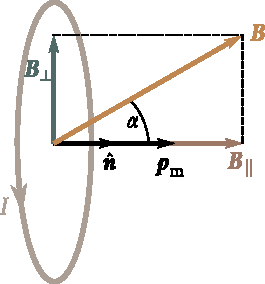
\includegraphics[scale=1]{figures/ch_06/fig_6_16.pdf}
		\caption[]{}
		\label{fig:6_16}
	\end{center}
	\vspace{-0.8cm}
\end{figure}

\noindent
Hình \fig{6_16} cho thấy
\begin{equation*}
    \ab{\vec{p}}{m} \times \vec{B}_{\perp} = \ab{\vec{p}}{m} \times \vec{B}.
\end{equation*}

\noindent
Do đó, trong trường hợp tổng quát, moment lực tác dụng lên một vòng dây kín đồng phẳng trong từ trường đồng nhất được xác định bởi phương trình \begin{equation}\label{eq:6_73}
    \vec{T} = \ab{\vec{p}}{m} \times \vec{B}.
\end{equation}

\noindent
Độ lớn của vector $\vec{T}$ là
\begin{equation}\label{eq:6_74}
    T = \ab{p}{m} B \sin\alpha.
\end{equation}

Để tăng góc a hợp giữa vector $\ab{\vec{p}}{m}$ và vector $\vec{B}$ một khoảng $\deriv{\alpha}$, công sau đây phải được thực hiện để chống lại lực từ tác dụng lên vòng dây đặt trong từ trường:
\begin{equation}\label{eq:6_75}
    \deriv{A} = T\, \deriv{\alpha} = \ab{p}{m} B \sin\alpha\, \deriv{\alpha}.
\end{equation}

\noindent
Khi trở lại vị trí ban đầu của nó, vòng dây có thể trả lại công dành cho việc làm quay nó bằng cách thực hiện công lên các các vật thể khác. Do đó, công trong phương trình \eqref{eq:6_75} làm tăng thế năng $\ab{W}{p,mech}$ mà một dòng điện kín có khi đặt trong từ trường bởi giá trị sau
\begin{equation*}
    \deriv{\ab{W}{p,mech}} = \ab{p}{m} B \sin\alpha\, \deriv{\alpha}.
\end{equation*}

\noindent
Tích phân phương trình trên, ta thu được
\begin{equation*}
    \ab{W}{p,mech} = - \ab{p}{m} B \cos\alpha + \text{constant}.
\end{equation*}

\noindent
Giả sử rằng $\text{constant}=0$, ta thu được biểu thức sau:
\begin{equation}\label{eq:6_76}
    \ab{W}{p,mech} = - \ab{p}{m} B \cos\alpha = - \ab{\vec{p}}{m} \ccdot \vec{B}
\end{equation}

\noindent
[So sánh với phương trình \eqn{6_61}].

Từ biểu thức \eqref{eq:6_76}, ta thấy rằng vị trí cực tiểu năng lượng, hay còn gọi là vị trí cân bằng bền, ứng với khi các vector $\ab{\vec{p}}{m}$ và $\vec{B}$ nằm song song và cùng chiều nhau

Đại lượng biểu diễn bởi \eqn{6_76} không đặc trưng cho tổng thế năng của vòng dây, mà chỉ là thành phần thế năng xuất hiện do moment lực tác dụng lên vòng, như được thấy ở \eqref{eq:6_73}. Để nhấn mạnh điều này, thế năng được biểu diễn trong \eqn{6_76} có thêm chỉ từ "mech". Tổng thế năng của vòng dây sẽ gồm nhiều số hạng khác ngoài $\ab{W}{p,mech}$.

Giờ chúng ta sẽ xem xét một dòng điện kín đồng phẳng đặt trong từ trường không đồng nhất. Chúng ta sẽ xét trường hợp dòng điện tròn để đơn giản hóa. Giả sử rằng từ trường thay đổi nhanh nhất theo hướng $x$ trùng với hướng của $\vec{B}$ tại tâm của dòng điện, và moment từ của vòng dây cũng hướng theo $\vec{B}$ (\fig{6_17}a).

\begin{figure}[t]
	\begin{center}
		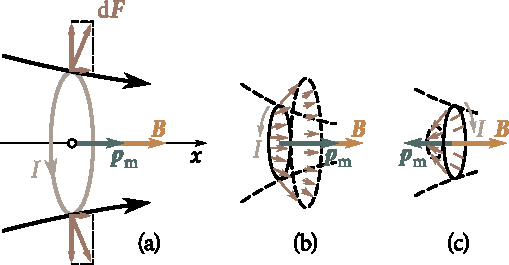
\includegraphics[scale=1]{figures/ch_06/fig_6_17.pdf}
		\caption[]{}
		\label{fig:6_17}
	\end{center}
	\vspace{-0.8cm}
\end{figure}

Ở đây, do $\vec{B}\neq\text{constant}$, nên \eqn{6_68} sẽ có thể khác không. Lực $\deriv{\vec{F}}$ tác dụng lên một phần tử dòng sẽ vuông góc với $\vec{B}$, \ie, với đường sức từ mà cắt $\deriv{\vec{l}}$. Do đó, các lực tác dụng lên các phần tử dòng khác nhau sẽ đều nằm trên một nón đối xứng (\fig{6_17}b). Lực tổng hợp $\vec{F}$ sẽ hướng theo chiều tăng của $\vec{B}$ và, do đó, có xu hướng kéo vòng dây vào vùng có từ trường lớn hơn. Dễ thấy rằng sự thay đổi của từ trường càng mạnh ($\diffinpartial{B}{x}$ càng lớn), thì góc đỉnh của nón nói trên sẽ càng nhỏ và, nếu các điều kiện khác không đổi, lực tổng hợp $\vec{F}$ sẽ càng lớn.
Nếu chúng ta đảo chiều dòng điện (giờ $\ab{\vec{p}}{m}$ song song ngược chiều với $\vec{B}$) thì hướng của các lực $\deriv{\vec{F}}$ và lực tổng hợp $\vec{F}$ sẽ bị đảo ngược (\fig{6_17}c). Do đó, với cách sắp xếp $\ab{\vec{p}}{m}$ và $\vec{B}$ như trên, vòng dây sẽ bị đẩy ra khỏi từ trường

Ta dễ dàng thu được biểu thức định lượng cho lực $\vec{F}$ bằng cách sử dụng \eqn{6_76} về năng lượng của vòng dây trong từ trường. Nếu hướng của moment từ so với từ trường là không đổi ($a=\text{constant}$), thì $\ab{W}{p,mech}$ sẽ chỉ phụ thuộc vào $x$ (thông qua $B$). Đạo hàm $\ab{W}{p,mech}$ theo $x$ và đổi dấu kết quả, ta thu được hình chiếu của lực lên trục $x$ là:
\begin{equation*}
    F_x = - \diffpartial{\ab{W}{p,mech}}{x} = \ab{p}{m} \diffpartial{B}{x} \cos\alpha.
\end{equation*}

\noindent
Nếu chúng ta giả thiết rằng từ trường thay đổi không đáng kể theo các phương còn lại thì ta có thể bỏ qua hình chiếu của lực lên các phương khác và đặt $F=F_x$. Vậy,
\begin{equation}\label{eq:6_77}
    F = \ab{p}{m} \diffpartial{B}{x} \cos\alpha.
\end{equation}

Từ phương trình ta thu được, ta thấy rằng lực tác dụng lên vòng dây có dòng điện được đặt trong từ trường không đều phụ thuộc vào cách sắp xếp moment từ của vòng dây so với hướng của từ trường. Nếu các vector $\ab{\vec{p}}{m}$ và $\vec{B}$ trùng hướng nhau ($\alpha=0$), thì lực là dương, \ie, hướng theo chiều tăng của $vec{B}$ ($\diffinpartial{B}{x}=0$ được giả thiết là dương; nếu không thì dấu và chiều của lực sẽ bị đảo ngược nhưng khi đó, lực vẫn có xu hướng kéo vòng dây vào vùng có từ trường mạnh như trước). Nếu $\ab{\vec{p}}{m}$ và $\vec{B}$ song song và ngược chiều nhau ($\alpha=\pi$), lực sẽ là âm, \ie, hướng theo chiều giảm của $\vec{B}$. Dựa trên hình \fig{6_17}, chúng ta cũng đã suy ra điều trên một cách định tính rồi.

Dễ dạng nhận thấy rằng dòng điện kín đặt trong từ trường không đều sẽ phải chịu tác dụng của cả lực, như được tính ở \eqref{eq:6_77}, và moment lực, như ta thấy ở \eqref{eq:6_73}.

\section{Từ trường của Dòng điện vòng}\label{sec:6_9}

Chúng ta hãy xem xét từ trường sinh ra bởi dòng điện chạy trong dây dẫn mảnh có dạng một vòng tròn bán kính $R$ (một dòng điện tròn). Ta sẽ xác định cảm ứng từ tại tâm vòng dây (\fig{6_18}). Tại tâm vòng, mọi phần tử dòng đều sinh ra cảm ứng từ có hướng vuông góc với mặt phẳng vòng dây. Do vậy, độ lớn của tổng vector của các $\deriv{\vec{B}}$ chính là tổng độ lớn của chúng. Từ \eqn{6_29},
\begin{equation*}
    \deriv{B} = \frac{\mu_0}{4\pi} \frac{I\, \deriv{l}}{R^2}
\end{equation*}

\noindent
($\alpha=\pi/2$). Tích phân biểu thức này trên toàn bộ vòng dây:
\begin{equation*}
    B = \int \deriv{B} = \frac{\mu_0}{4\pi} \frac{I}{R^2} \oint \deriv{l} = \frac{\mu_0}{4\pi} \frac{I}{R^2} 2\pi R = \frac{\mu_0}{4\pi} \frac{2I \parenthesis{\pi R^2}}{R^3}.
\end{equation*}

Biểu thức trong ngoặc là độ lớn của moment từ $\ab{p}{m}$ [xem lại \eqn{6_71}]. Do vậy, cảm ứng từ tại tâm dòng điện tròn có độ lớn là
\begin{equation}\label{eq:6_78}
    B = \frac{\mu_0}{4\pi} \frac{2\ab{p}{m}}{R^3}.
\end{equation}

Xem xét \fig{6_18}, ta thấy được rằng hướng của vector $\vec{B}$ trùng với hướng vector pháp tuyến của mặt phẳng vòng dây, \ie, với hướng của vector $\ab{\vec{p}}{m}$. Do vậy, \eqn{6_78} có thể được viết dưới dạng vector:
\begin{equation}\label{eq:6_79}
    \vec{B} = \frac{\mu_0}{4\pi} \frac{2\ab{\vec{p}}{m}}{R^3}.
\end{equation}

\begin{figure}[t]
	\begin{minipage}[t]{0.35\linewidth}
		\begin{center}
			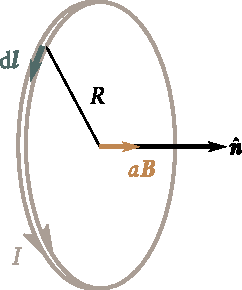
\includegraphics[scale=0.98]{figures/ch_06/fig_6_18.pdf}
			\caption[]{}
			\label{fig:6_18}
		\end{center}
	\end{minipage}
	\hfill{ }%space{-0.05cm}
	\begin{minipage}[t]{0.61\linewidth}
		\begin{center}
			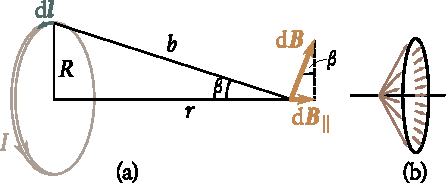
\includegraphics[scale=0.98]{figures/ch_06/fig_6_19.pdf}
			\caption[]{}
			\label{fig:6_19}
		\end{center}
	\end{minipage}
\vspace{-0.4cm}
\end{figure}

Giờ chúng ta sẽ tính  $\vec{B}$ tại một điểm trên trục của vòng dây, cách tâm vòng dây một đoạn $r$ (\fig{6_19}). Các vector  $\deriv{\vec{B}}$ pháp tuyển với mặt phẳng chứa phần tử dòng $\deriv{\vec{l}}$ và điểm mà chúng ta đang xét. Do đó, các vector này nằm trên một hình nón đối xứng. (\fig{6_19}b). Do tính đối xứng, ta có thể kết luận rằng vector tổng hợp $\vec{B}$ có hướng dọc theo trục của vòng dây.
Mỗi phần tử vector $\deriv{\vec{B}}$ đóng góp  $\deriv{\vec{B}_{parallel}}$ có độ lớn là $\deriv{B}\sin\beta=\deriv{B}(R/b)$ cho vector tổng hợp. Góc $\alpha$ hợp giữa vector $\deriv{\vec{l}}$ và vector $\vec{b}$ là góc vuông, do đó : 
\begin{equation*}
    \deriv{B_{\parallel}} = \deriv{B} \frac{R}{b} = \frac{\mu_0}{4\pi} \frac{I\, \deriv{l}}{b^2} \frac{R}{b} = \frac{\mu_0}{4\pi} \frac{I R\, \deriv{l}}{b^3}.
\end{equation*}

\noindent
Tích phân phương trình cho toàn bộ vòng dây và thay thể $\sqrt{R^2+r^2}$ bởi $b$, ta thu được 
\begin{align}
    B &= \int \deriv{B_{\parallel}} = \frac{\mu_0}{4\pi} \frac{I R}{b^3} \oint \deriv{l} = \frac{\mu_0}{4\pi} \frac{I R}{b^3} 2\pi R = \frac{\mu_0}{4\pi} \frac{2\parenthesis{I \pi R^2}}{\parenthesis{R^2+r^2}^{3/2}} \nonumber\\
    &= \frac{\mu_0}{4\pi} \frac{2 \ab{p}{m}}{\parenthesis{R^2+r^2}^{3/2}}. \label{eq:6_80}
\end{align}

\noindent
Biểu thức này xác định độ lớn của cảm ứng từ tại một điểm trên trục của vòng dây. Khi mà $\vec{B}$ và $\ab{\vec{p}}{m}$ cùng hướng, ta có thể viết phương trình \eqn{6_80} dưới dạng vector:
\begin{equation}\label{eq:6_81}
    \vec{B} = \frac{\mu_0}{4\pi} \frac{2 \ab{\vec{p}}{m}}{\parenthesis{R^2+r^2}^{3/2}}.
\end{equation}

\noindent
Biểu thức này không phụ thuốc vào dấu của $r$. Do đó, ở các điểm có đối xứng trục với nhau qua tâm của dòng điện,  $\vec{B}$ có cùng độ lớn và hướng.

Khi $r=0$, phương trình \eqn{6_81}, như dự đoán, trở thành biểu thức \eqn{6_79} cho cảm ứng từ tại tâm của một dòng điện tròn.

Ở những điểm cách xa vòng dây, ta có thể bỏ qua thành phần $R^2$ trong mẫu số, và khi đó phương trình \eqref{eq:6_81} trở thành
\begin{equation}\label{eq:6_82}
    \vec{B} = \frac{\mu_0}{4\pi} \frac{2 \ab{\vec{p}}{m}}{r^3}\quad (\text{along the current axis}),
\end{equation}

\noindent
giống như biểu thủc \eqn{1_55} xác định cường độ điện tường trên trục của một lưỡng cực điện.

Các tính toán nằm ngoài phạm vi của sách cho thấy rằng ta có thể thiết lập moment lưỡng cực từ $\ab{\vec{p}}{m}$ cho mọi hệ các dòng điện hay điện tích chuyển động mà bị giới hạn trong một vùng không gian hữu hạn (tương tự như moment lưỡng cực điện cho một nhóm các điện tích). Công thức liên hệ giữa từ trường của hệ trên ở khoảng cách rất lớn so với kích cỡ của hệ và $\ab{\vec{p}}{m}$ cũng tương tự với công thức liên hệ giữa điện trường của nhóm các điện tích tại một điểm cách rất xa nhóm và moment lưỡng cực điện (xem lại \sect{1_10}). Cụ thể, từ trường của vòng dây đồng phẳng có hình dạng bất kì ở điểm cách rất xa vòng dây sẽ là
\begin{equation}\label{eq:6_83}
    B = \frac{\mu_0}{4\pi} \frac{2 \ab{p}{m}}{r^3} \sqrt{1 + 3 \cos^2\theta},
\end{equation}

\noindent
trong đó $r$ là khoảng cách từ vòng dây đến điểm được chọn, và $\theta$ là góc tạo bởi hướng của vector $\ab{\vec{p}}{m}$ và hướng từ vòng dây đến điểm này [có thể so sánh với \eqn{1_53}]. Khi $\theta=0$, \eqn{6_83} sẽ cho kết quả giống với \eqn{6_82} về độ lớn của vector $\vec{B}$.

\begin{figure}[t]
	\begin{center}
		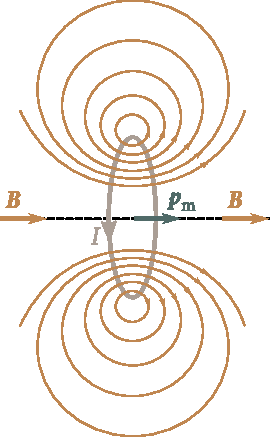
\includegraphics[scale=1]{figures/ch_06/fig_6_20.pdf}
		\caption[]{}
		\label{fig:6_20}
	\end{center}
	\vspace{-0.8cm}
\end{figure}

Hình \ref{fig:6_20} cho thấy các đường sức từ của dòng điện tròn. Hình trên chỉ biểu diễn các đường sức từ nằm trong một trong các mặt phẳng đi qua trục của dòng điện vì hình vẽ đường sức từ trong các mặt phẳng còn lại sẽ không khác gì so với hình này.

Qua chương trước và chương này, chúng ta có thể thấy rằng moment lưỡng cực từ là một thông số rất quan trọng của một dòng điện vòng vì nó giúp chúng ta biết được từ trường sinh ra bởi vòng cũng như ảnh hưởng của từ trường lên vòng đó.

\section{Công thực hiện khi một dòng điện chuyển động trong từ trường}\label{6_10}

Xét một dòng điện kín tạo bởi các dây dẫn cố định và một thanh di động có chiều dài $l$ trượt trên khung dây đó (\fig{6_21}). Đặt khung dây trong từ trường ngoài đồng nhất có phương vuông góc với mặt phẳng của khung dây. Với hướng của dòng điện và từ trường như hình vẽ. Với hướng của dòng điện và từ trường như hình vẽ, lưc $\vec{F}$ tác dụng lên thanh sẽ hướng về bên phải và có độ lớn là
\begin{equation*}
    F = I B l.
\end{equation*}

\noindent
Khi thanh di chuyển sang bên phải một đoạn $\deriv{h}$, lực này thực hiện công dương bằng
\begin{equation}\label{eq:6_84}
    \deriv{A} = F\, \deriv{h} = I B l\, \deriv{h} = I B\, \deriv{S},
\end{equation}

\noindent
trong đó $\deriv{S}$ ứng với vùng được tô màu (xem \fig{6_21}a).

Hãy xem xét từ thông $\Phi$ qua khung dây thay đổi như nào khi mà thanh chuyển động Khi tính từ thông qua diện tích khung dây, ta giả sử vector $\hatvec{n}$ trong phương trình
\begin{equation*}
    \Phi = \int \vec{B} \ccdot \hatvec{n}\, \deriv{S},
\end{equation*}

\noindent
là vector pháp tuyến theo chiều dương, ( vector xác định thông qua dòng điện bởi quy tắc nắm tay phải ) (xem  \sect{6_8}). Do đó, trong trường hợp của hình \fig{6_21}a, từ thông sẽ có giá trị dương và có giá trị là $BS$ ($S$ là diện tích của khung dây ). Khi thanh di chuyển về bên phải, diện tích của khung dây thay đổi 1 khoảng $\deriv{S}$. Vì thế, từ thông qua khung dây cũng tăng lên 1 đoạn $\deriv{\Phi}=B\,\deriv{S}$. Phương trình  \eqref{eq:6_84} do đó, có thể được viết dưới dạng
\begin{equation}\label{eq:6_85}
    \deriv{A} = I\, \deriv{\Phi}.
\end{equation}

\begin{figure}[t]
	\begin{center}
		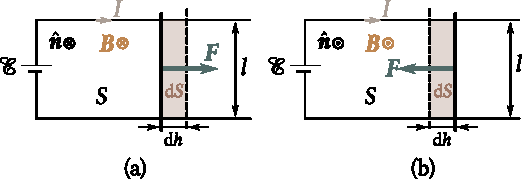
\includegraphics[scale=1.1]{figures/ch_06/fig_6_21.pdf}
		\caption[]{}
		\label{fig:6_21}
	\end{center}
	\vspace{-0.8cm}
\end{figure}

\noindent
Khi từ trường hướng ra khỏi mặt phẳng (\fig{6_21}b), lực tác dụng lên thanh có hướng vê phia bên trai. Do đó, khi mà thanh chuyển động về phía bên phải một đoạn $\deriv{h}$, lực từ thực hiện công âm \begin{equation}\label{eq:6_86}
    \deriv{A} = - I B l\, \deriv{h} = - I B\, \deriv{S}.
\end{equation}

\noindent
Trong trường hợp này, từ thông qua khung dây có giá trị là $-BS$. Khi diện tích của khung dây tăng một khoảng $\deriv{S}$, từ thông biến đổi 1 đoạn $\deriv{\Phi}=-B\,\deriv{S}$. Do đó, phương trình \eqn{6_86} có thể được viết dưới dạng của phương trình \eqn{6_85}.

Đại lượng $\deriv{\Phi}$ trong phương trình \eqn{6_85} là từ thông qua vùng diện tích mà thanh đi qua trong quá trình chuyển động. Tương tự, ta có thể nói công thực hiện bởi lực từ trên 1 phần của dòng điện kín bằng tích của dòng điện và từ thông qua diện tích mà phần này đi qua trong quá trình chuyển động.

Các biểu thức \eqref{eq:6_84} và \eqref{eq:6_85} có thể được gộp thành một biểu thức vector. Để làm điều này, chúng ta sẽ so sánh vector $\vec{l}$ có hướng của dòng điện với thanh (\fig{6_22}). Với hướng bất kì của vector $\vec{B}$ (hướng vào hay hướng ra khỏi chúng ta), lực tác dụng lên thanh có thể được biểu diễn là
\begin{equation*}
    \vec{F} = I \vecprod{l}{B}.
\end{equation*}

\noindent
Khi thanh di chuyển một đoạn $\derivec{h}$, lực thực hiện công
\begin{equation*}
    \deriv{A} = \vec{F}\, \derivec{h} = I \vecprod{l}{B}\, \derivec{h}.
\end{equation*}

\noindent
Chúng ta sẽ thay đổi các nhân tử trong tích vô hướng bội ba trên [xem lại Eq. (1.34) của Vol. I]. Khi đó, ta thu được
\begin{equation}\label{eq:6_87}
    \deriv{A} = I \vec{B} (\derivec{h} \times \vec{l}).
\end{equation}

\begin{figure}[t]
	\begin{center}
		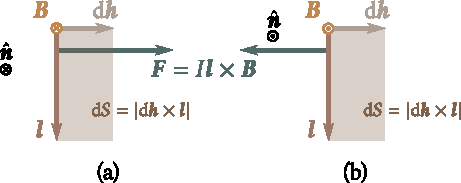
\includegraphics[scale=1.1]{figures/ch_06/fig_6_22.pdf}
		\caption[]{}
		\label{fig:6_22}
	\end{center}
	\vspace{-0.8cm}
\end{figure}

Nhìn qua \fig{6_22}, ta thấy được rằng tích vector $(\derivec{h}\times\vec{l})$ có độ lớn bằng với diện tích $\deriv{S}$ được bao bởi thanh trong khi nó chuyển động và có hướng của vector pháp tuyến $\hatvec{n}$. Do vậy,
\begin{equation}\label{eq:6_88}
    \deriv{A} = I (\vec{B} \ccdot \hatvec{n})\, \deriv{S}.
\end{equation}

\noindent
Trong trường hợp được miêu tả ở \fig{6_22}a, ta có $\vec{B}\ccdot\hatvec{n}=B$, và ta nhận được \eqn{6_84}. Trong trường hợp ở \fig{6_22}b, ta lại có $\vec{B}\ccdot\hatvec{n}=-B$ và do đó ta thu được \eqn{6_86}.

Độ thay đổi của từ thông qua dòng điện kín do sự chuyển động của thanh là $\vec{B}\ccdot\hatvec{n}\,\deriv{S}$ . Do vậy, \eqn{6_88} có thể được viết lại thành \eqref{eq:6_85}. Tuy nhiên sử dụng \eqn{6_88} có lợi hơn so với việc sử dụng \eqref{eq:6_85} vì khi đó chúng ta sẽ ``tự động'' có được dấu của $\deriv{\Phi}$ cũng như dấu của $\deriv{A}$.

Chúng ta hãy xem xét một dòng điện kín và có hình dạng tùy ý không đổi đặt trong từ trường bất kì. Ta sẽ tìm công tác dụng lên một phần tử dây vô cùng nhỏ trong đó. Giả sử phần từ dây $\derivec{l}$ chuyển dời một đoạn $\derivec{h}$ (\fig{6_23}). Công mà lực từ thực hiện lên nó là:
\begin{equation}\label{eq:6_89}
    \deriv{\ab{A}{el}} = I (\derivec{l} \times \vec{B}) \ccdot \derivec{h}.
\end{equation}

\noindent
Ở đây, $\vec{B}$ là cảm ứng từ tại vị trí của phần tử dòng $\derivec{l}$.

Đảo vị trí các nhân tử trong \eqn{6_89}, ta được
\begin{equation}\label{eq:6_90}
    \deriv{\ab{A}{el}} = I \vec{B} \ccdot (\derivec{h} \times \derivec{l}).
\end{equation}

\noindent
Giá trị của tích vector $\derivec{h} \times\derivec{l}$ bằng với diện tích của hình bình hành tạo bởi $\derivec{h}$ và $\derivec{l}$, tương đương với diện tích mà vector $\derivec{l}$ quét qua trong quá trinh chuyển động. Hướng của vector này trùng với hướng của chiều dương vector pháp tuyến của diện tích $\deriv{S}$. Do đó.
\begin{equation}\label{eq:6_91}
    \vec{B} \ccdot (\derivec{h} \times \derivec{l}) = (\vec{B} \ccdot \hatvec{n})\, \deriv{S} = \deriv{\ab{\Phi}{el}},
\end{equation}

\noindent
trong đó $\deriv{\ab{\Phi}{el}}$ là độ biến thiên của từ thông qua vòng dây do sự dịch chuyển của phần tử vòng dây $\derivec{l}$.

\begin{figure}[t]
	\begin{center}
		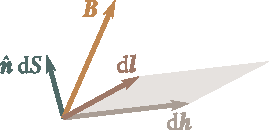
\includegraphics[scale=0.98]{figures/ch_06/fig_6_23.pdf}
		\caption[]{}
		\label{fig:6_23}
	\end{center}
	\vspace{-0.9cm}
\end{figure}

Theo phương trình \eqn{6_91}, ta có thể viết lại phương trình \eqn{6_90} dưới dạng 
\begin{equation}\label{eq:6_92}
    \deriv{\ab{A}{el}} = I\, \deriv{\ab{\Phi}{el}}.
\end{equation}

\noindent
Tổng của phương trình \eqn{6_92} với tất cả các phân tử của vòng dây cho ta  biểu thức của công lực từ sau một dịch chuỷen rất nhỏ của vòng dây:  
\begin{equation}\label{eq:6_93}
    \deriv{A} = \int \deriv{\ab{A}{el}} = \int I \, \deriv{\ab{\Phi}{el}} = I \int \deriv{\ab{\Phi}{el}} = I\, \deriv{\Phi}
\end{equation}

\noindent
($\deriv{\Phi}$  là tổng độ biến thiên từ thông qua vòng dây).

Để xác định công thực hiện lên một vòng dây thực hiện dịch chuyển đáng kể, ta tích phân phương trình \eqn{6_93} trên toàn bộ vòng dây:
\begin{equation}\label{eq:6_94}
    A_{12} = \int \deriv{A} = I \int \deriv{\ab{\Phi}{el}} = I \parenthesis{\Phi_2 - \Phi_1}.
\end{equation}

\noindent
Ở đây, $\Phi_1$ và $\Phi_2$ là các giá trị của từ thông qua vòng dây lần lượt ở vị trí ban đầu và vị trí cuối cùng của nó. Do vậy, công thực hiện bởi lực từ lên vòng dây trên sẽ bằng với tích của dòng điện với sự thay đổi của từ thông qua vòng.

Cụ thể, khi một vòng dây đồng phẳng đặt trong một trường đều quay từ vị trí mà các vector $\ab{\vec{P}}{m}$ và $\vec{B}$ ngược chiều nhau (ở vị trí này $\Phi=-BS$) tới vị trí mà tại đó hai vector trên cùng chiều nhau (lúc này $\Phi=BS$), công do lực từ tác dụng lên vòng dây sẽ là:
\begin{equation*}
    A = I [BS - (BS)] = 2 I B S.
\end{equation*}

\noindent
Ta sẽ thu được kết quả tương tự nếu sử dụng \eqn{6_91} dành cho thế năng của vòng dây trong từ trường:
\begin{equation*}
    A = \ab{W}{init} - \ab{W}{fin} = \ab{p}{m} B - (- \ab{p}{m} B) = 2 \ab{p}{m} B = 2 I S B
\end{equation*}

\noindent
($\ab{p}{m}=IS$).

Lưu ý rằng công được biểu diễn bởi phương trình \eqn{6_94} không thực sự được thực hiện bởi từ trường ngoài, mà là bởi nguồn điện được sử dụng để duy trì dòng điện không đổi qua vòng dây. Trong phần \sect{8_2}, ta sẽ cho thấy rằng khi từ thông qua một vòng dây thay đổi, một suất điện động cảm ứng $\ab{\mathcal{E}}{i}=-(\diffin{\Phi}{t})$ sẽ xuất hiện trong vòng dây trên. Do vậy, nguồn điện không chỉ phải sinh công để giải phóng nhiệt lượng Joule mà còn phải sinh công để chống lại suất điện động trên. Biểu thức của công thực hiện bởi nguồn là 
\begin{equation*}
    A = \int \deriv{A} = -\int \ab{\mathcal{E}}{i} l\, \deriv{t} = \int \diffin{\Phi}{t} I\, \deriv{t} = \int I\, \deriv{\Phi} = I (\Phi_2 - \Phi_1),
\end{equation*}

\noindent
, giống với \eqn{6_94}.

\section{Divergence và Curl của Từ trường}\label{sec:6_11}

Do không tồn tại từ tích trong tự nhiên\footnote{Nhà vật lý học người Anh Paul Dirac đã giả sử rằng các từ tích (được gọi là đơn cực từ Dirac) có tồn tại trong tự nhiên. Tuy vậy, mọi nỗ lực tìm kiếm các từ tích trên đều không đưa ra kết quả} nên các đường sức từ của $\vec{B}$ không có điểm đầu hay điểm kết. Dựa trên \eqn{1_77}, ta thấy rằng thông lượng của $\vec{B}$ qua một mặt kín phải bằng không. Vậy, với từ trường và mặt kín bất kì, điều kiện
\begin{equation}\label{eq:6_95}
    \Phi_B = \oint_S \vec{B}\, \derivec{S} = 0,
\end{equation}

\noindent
phải thỏa mãn. Phương trình trên biểu diễn định luật Gauss cho $\vec{B}$: từ thông qua một mặt kín bất kì sẽ bằng không.

Thay tích phân mặt trong \eqn{6_95} bằng một tích phân thể tích sao cho phù hợp với \eqn{1_108}, ta sẽ thấy được là
\begin{equation*}
    \int_V \divop{\vec{B}}\, \deriv{V} = 0.
\end{equation*}

\noindent
Điều kiện trên phải thỏa mãn với vùng thể tích $V$ bất kì. Điều này chỉ xảy ra nếu như hàm bên trong tích phân bằng không tại mọi điểm trong không gian. Vậy, div của từ trường bằng không ở mọi nơi: 
\begin{equation}\label{eq:6_96}
    \divop{\vec{B}} = 0.
\end{equation}

Giờ chúng ta sẽ xem xét lưu số của vector $\vec{B}$. Từ định nghĩa, lưu số bằng với tích phân sau
\begin{equation}\label{eq:6_97}
    \oint \vec{B} \ccdot \derivec{l}.
\end{equation}

\noindent
Chúng ta sẽ xem xét tích phân trên với từ trường của dòng điện thẳng do khi đó, rất dễ tính tích phân trên. Giả sử rằng có một vòng kín nằm trong mặt phẳng vuông góc với chiều dòng điện (\fig{6_24}; dòng điện vuông góc với mặt phẳng hình vẽ và hướng ra ngoài hình vẽ). Tại mỗi điểm của vòng kín trên, vector $\vec{B}$ có hướng tiếp tuyến với chu vi đường tròn có tâm ở trên dây và đi qua điểm này. Chúng ta sẽ dùng $B\,\deriv{l_B}$ thay cho $\vec{B}\ccdot \derivec{l}$ trong biểu thức của lưu số ($\deriv{l_B}$ là hình chiếu của một phần tử vòng lên vector $\vec{B}$). Từ hình vẽ, ta thấy $\deriv{l_B}$ bằng $b\,\deriv{\alpha}$, trong đó $b$ là khoảng cách từ dây mang dòng điện đến $\derivec{l}$, và $\deriv{\alpha}$ là góc quay của đường nối tâm khi ta di chuyển dọc theo phần tử $\derivec{l}$.
Vậy, thay biểu thức \eqn{6_30} dành cho $B$ vào, ta được
\begin{equation}\label{eq:6_98}
    \vec{B} \ccdot \derivec{l} = B\,\deriv{l_B} = \frac{\mu_0}{4\pi} \frac{2I}{b} b\, \deriv{\alpha} = \frac{\mu_0 I}{2\pi}\, \deriv{\alpha}.
\end{equation}

\begin{figure}[t]
	\begin{center}
		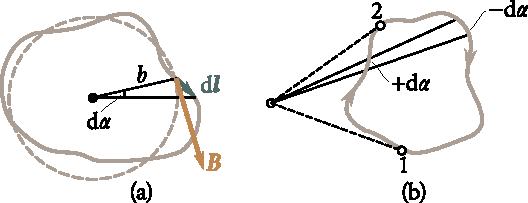
\includegraphics[scale=1.0]{figures/ch_06/fig_6_24.pdf}
		\caption[]{}
		\label{fig:6_24}
	\end{center}
	\vspace{-0.8cm}
\end{figure}

Từ \eqn{6_98}, ta có
\begin{equation}\label{eq:6_99}
    \oint \vec{B} \ccdot \derivec{l} = \frac{\mu_0 I}{2\pi} \oint \deriv{\alpha}.
\end{equation}

\noindent
Sau khi chúng ta đi quanh vòng kín, ta thấy rằng đường nối tâm liên tục quay theo một chiều, do đó, $\oint\deriv{\alpha}= 2\pi$. Kết quả sẽ khác nếu vòng kín trên không bao lấy dòng điện (\fig{6_24}b). Khi đó, trong khi đi quanh vòng, đường nối tâm lúc đầu sẽ quay theo một chiều (đoạn $1$-$2$), và rồi quay theo chiều còn lại ($2$-$1$), dẫn tới $\oint\deriv{\alpha}$ bằng không. Dựa trên kết quả trên, ta có thể viết là
\begin{equation}\label{eq:6_100}
    \oint \vec{B} \ccdot \derivec{l} = \mu_0 I,
\end{equation}

\noindent
trong đó $I$ là dòng điện được bao bởi vòng kín trên. Nếu vòng kín do ta chọn không bao quanh dòng điện, lưu số của vector $\vec{B}$ sẽ là không.

Dấu của biểu thức \eqref{eq:6_100} phụ thuộc vào chiều quay quanh vòng kín (góc $\alpha$ sẽ được đo theo chiều trên). Nếu hướng quay quanh vòng tạo thành một tam diện thuận với hướng của dòng điện thì đại lượng \eqref{eq:6_100} là dương, còn trong trường hợp ngược lại thì nó là âm. Ta có thể xác định dấu trong biểu thức bằng cách coi $I$ như một đại lượng đại số. Nếu chiều dòng điện và chiều quay theo vòng kín liên hệ với nhau qua quy tắc nắm tay phải thì giá trị của $I$ là dương; dòng điện có chiều ngược lại sẽ có giá trị âm.

Phương trình \eqref{eq:6_100} sẽ giúp chúng ta dễ dàng nhớ lại \eqn{6_30} cho từ trường $B$ của dòng điện thẳng. Tưởng tượng có một vòng kín đồng phẳng có dạng đường tròn bán kính $b$ (\fig{6_25}). Tại mọi điểm trên vòng kín này, vector $\vec{B}$ đều có cùng độ lớn và hướng theo phương tiếp tuyến của đường tròn. Do đó, lưu số sẽ bằng với tích của $B$ và độ dài chu vi $2\pi b$, và \eqn{6_100} sẽ có dạng
\begin{equation*}
    B \times 2\pi b = \mu_0 I.
\end{equation*}

\noindent
Từ đây ta được $B=\mu_0 I/(2\pi b)$ [giống với \eqn{6_30}].

\begin{figure}[t]
	\begin{minipage}[t]{0.41\linewidth}
		\begin{center}
			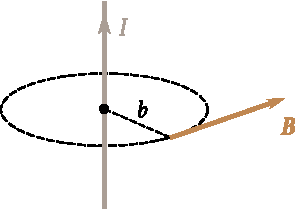
\includegraphics[scale=1]{figures/ch_06/fig_6_25.pdf}
			\caption[]{}
			\label{fig:6_25}
		\end{center}
	\end{minipage}
	\hfill{ }%space{-0.05cm}
	\begin{minipage}[t]{0.55\linewidth}
		\begin{center}
			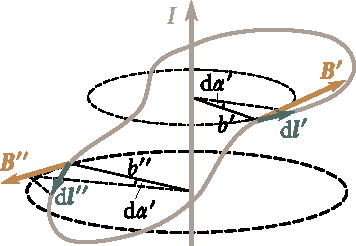
\includegraphics[scale=1]{figures/ch_06/fig_6_26.pdf}
			\caption[]{}
			\label{fig:6_26}
		\end{center}
	\end{minipage}
\vspace{-0.4cm}
\end{figure}

Trong trường hợp vòng kín được chọn là không đồng phẳng (\fig{6_26}), ta thấy rằng đường nối tâm lúc này sẽ không chỉ quay quanh dây mà còn di chuyển dọc theo dây nữa. Khi đó, mọi lập luận ta đã sử dụng để có được \eqn{6_100} vẫn sẽ đúng nếu ta hiểu $\deriv{\alpha}$ là góc quay của hình chiếu của đường nối tâm lên mặt phẳng vuông góc với dòng điện. Góc quay của hình chiếu này là $2\pi$ nếu như vòng kín bao quanh dòng điện, và bằng không nếu vòng kín không chứa dòng điện. Vậy chúng ta lại thu được \eqn{6_100}.

Ta đã chứng minh được \eqn{6_100} cho dòng điện thẳng. Ta có thể chứng minh rằng công thức trên vẫn đúng cho các dòng điện có dạng khác, chẳng hạn như dòng điện tròn.

Giả sử rằng vòng kín ta chọn bao lấy nhiều dây mang dòng điện. Từ nguyên lý chồng chập [xem lại \eqn{6_16}]:
\begin{equation*}
    \oint \vec{B}\ccdot \derivec{l} = \oint \parenthesis{ \sum_k \vec{B}_k }\, \derivec{l} = \sum_k \oint \vec{B}_k\, \derivec{l}.
\end{equation*}

\noindent
Mỗi tích phân trong tổng trên bằng với $\mu_0I_k$. Do đó,
\begin{equation}\label{eq:6_101}
    \oint \vec{B}\ccdot \derivec{l} = \mu_0 \sum_k I_k
\end{equation}

\noindent
(lưu ý rằng $I_k$ là một đại lượng đại số).

Nếu có dòng chạy trong toàn không gian quanh vị trí của vòng kín, tổng đại số của các dòng điện được bao bởi vòng sẽ có thể được biểu diễn dưới dạng
\begin{equation}\label{eq:6_102}
    \sum_k I_k = \int_S \vec{j}\ccdot \derivec{S} = \int_S \vec{j}\ccdot \hatvec{n}\, \deriv{S}.
\end{equation}

\noindent
Tích phân trên được lấy qua mặt $S$ bất kì được bao bởi vòng. Vector $\vec{j}$ là mật độ dòng điện ở vị trí của phần tử diện tích $\deriv{S}$; $\hatvec{n}$ là vector pháp tuyến của phần tử trên và hướng theo chiều dương (\ie, là vector pháp tuyến mà liên hệ với chiều quay quanh vòng kín để tính lưu số qua quy tắc bàn tay phải).

Thay \eqn{6_102} cho tổng dòng điện trong \eqn{6_101}, ta có 
\begin{equation*}
    \oint \vec{B}\ccdot \derivec{l} = \mu_0 \int_S \vec{j}\ccdot \derivec{S}.
\end{equation*}

Từ định luật Stokes, ta biến đổi vế trái của phương trình trên và thu được
\begin{equation*}
    \int_S (\curlop{\vec{B}}) \ccdot \derivec{S} = \mu_0 \int_S \vec{j}\ccdot \derivec{S}.
\end{equation*}

\noindent
Biểu thức trên phải đúng với mọi mặt $S$ được chọn để tính tích phân. Điều này chỉ khả thi nếu các hàm được tích phân như nhau tại mọi điểm. Vậy, chúng ta kết luận rằng curl của vector cảm ứng từ tại một điểm sẽ tỉ lệ thuận với mật độ khối dòng điện tại điểm đó:
\begin{equation}\label{eq:6_103}
    \curlop{\vec{B}} = \mu_0 \vec{j}.
\end{equation}

\noindent
Hệ số tỉ lệ trong hệ đơn vị SI là $\mu_0$.

Lưu ý rằng \eqns{6_101}{6_103} chỉ đúng cho từ trường trong chân không khi không có sự xuất hiện của điện trường biến thiên theo thời gian.

Vậy ta đã tìm được div và curl của từ trường trong chân không. Chúng ta sẽ so sánh các kết quả trên với các kết quả tương tự cho điện trường. Từ phương trình \eqref{eq:1_112}, \eqref{eq:1_117}, \eqref{eq:6_96} và \eqref{eq:6_103}:
\begin{align*}
    \divop{\vec{E}} = \frac{1}{\varepsilon_0}\rho &\quad \text{(div của $\vec{E}$ bằng $\rho$ chia cho $\varepsilon_0$)}\\
    \curlop{\vec{E}} = 0 &\quad \text{(curl của $\vec{E}$ bằng không)}\\
    \divop{\vec{B}} = 0 &\quad \text{(div của $\vec{B}$ bằng không)}\\
    \curlop{\vec{B}} = \mu_0 \vec{j} &\quad \text{(curl của $\vec{B}$ bằng $\mu_0$ nhân với $\vec{j}$)}.
\end{align*}

So sánh các phương trình trên với nhau sẽ cho ta thấy rằng từ trường và điện trường tĩnh có bản chất khác nhau. Curl của điện trường tĩnh bằng không; do vậy, điện trường tĩnh là trường thế và có thể được biểu diễn thông qua điện thế vô hướng $\varphi$. Curl của từ trường tại các điểm có dòng điện là khác không và lưu số của vector $\vec{B}$ tỉ lệ thuận với cường độ dòng điện được bao bởi vòng kín. Đây là lí do vì sao chúng ta không thể thiết lập một hàm thế vô hướng cho từ trường mà liên hệ với $\vec{B}$ qua một phương trình có dạng tương tự \eqn{1_41}. Nếu làm vậy thì hàm thế này sẽ không đơn trị---sau mỗi lần quay quanh vòng kín và trở về điểm đầu, hàm thế sẽ tăng thêm một lượng là $\mu_0 I$. Trường mà có curl khác không được gọi là \textbf{trường xoáy} hay  \textbf{trường solenoid}.

Do div của vector $\vec{B}$ bằng không ở mọi điểm nên vector này có thể được biểu diễn như là curl của một hàm $\vec{A}$:
\begin{equation}\label{eq:6_104}
    \vec{B} = \curlop{\vec{A}},
\end{equation}

\noindent
do div của curl luôn bằng không [xem lại \eqn{1_106}]. Hàm $\vec{A}$ được gọi là \textbf{thế vector}. Chúng ta sẽ không đi sâu vào thế vector do nó nằm ngoài phạm vi của cuốn sách hiện tại.

\section{Từ trường của Solenoid và Toroid}\label{sec:6_12}

Cuộn solenoid là một dây dẫn được cuốn lại thành hình xoắn ốc quanh một hình trụ tròn. Các đường sức từ của một cuộn solenoid có dạng xấp xỉ như \fig{6_27}. Hướng của các đường sức từ bên trong solenoid liên hệ với chiều dòng điện trong cuộn dây qua quy tắc bàn tay phải.

Trong thực tế, một cuộn solenoid sẽ luôn có thành phần dòng điện hướng dọc theo trục của nó. ngoài ra, mật độ dài của dòng điện $\ab{j}{lin}$ (bằng với tỉ số của cường độ dòng $\deriv{I}$ với chiều dài của một phần tử solenoid $\deriv{l}$) biến đổi tuần hoàn dọc theo solenoid. Giá trị trung bình của mật độ dài là
\begin{equation}\label{eq:6_105}
    \average{\ab{j}{lin}} = \average{\diff{I}{l}} = nI,
\end{equation}

\noindent
trong đó $n$ là số vòng của solenoid trên một đơn vị độ dài và $I$ là cường độ dòng điện chạy qua solenoid.

Trong điện từ học, việc khảo sát một solenoid dài vô tận, không có thành phần dòng hướng theo trục và có mật độ dài của dòng $\ab{j}{lin}$ không đổi xuyên suốt chiều dài của solenoid là rất quan trọng. Lý do là vì từ trường tạo bởi solenoid trên là đồng nhất và bị giới hạn bên trong solenoid (tương tự với việc điện trường sinh ra bởi tụ điện phẳng rộng vô hạn là đồng nhất và bị giới hạn bên trong tụ điện).

Vậy chúng ta hãy tưởng tượng rằng có một solenoid có dạng một mặt trụ vô cùng mỏng và có mật độ dài dòng điện không đổi chạy quanh
\begin{equation}\label{eq:6_106}
    \ab{j}{lin} = nI.
\end{equation}

\noindent
Ta sẽ chia mặt trụ trên thành các dòng điện tròn giống hệt nhau---gọi là vòng. Từ \fig{6_28}, ta thấy rằng một cặp vòng đặt đối xứng nhau qua mặt phẳng vuông góc với trục của solenoid sẽ sinh ra tại mọi điểm trên mặt phẳng này một vector cảm ứng từ tổng hợp có hướng song song với trục . Do vậy, từ trường ở mọi điểm, dù ở bên trong hay bên ngoài solenoid vô tận này, đều phải hướng song song với trục của solenoid.

Ta thấy từ \fig{6_27} rằng hướng của từ trường bên trong và bên ngoài solenoid hữu hạn là ngược chiều nhau. Hướng của từ trường không thay đổi khi ta thay đổi chiều dài của solenoid, vậy nên khi xét trường hợp giới hạn $l\to\infty$, hướng của chúng vẫn phải ngược nhau. Trong một solenoid vô tận, giống như với solenoid hữu hạn, hướng của từ trường trong cuộn solenoid phải liên hệ với chiều dòng điện chạy quanh cuộn qua quy tắc bàn tay phải.

\begin{figure}[t]
	\begin{minipage}[t]{0.48\linewidth}
		\begin{center}
			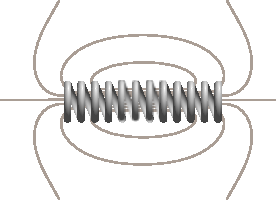
\includegraphics[scale=1]{figures/ch_06/fig_6_27b.pdf}
			\caption[]{}
			\label{fig:6_27}
		\end{center}
	\end{minipage}
	\hfill{ }%space{-0.05cm}
	\begin{minipage}[t]{0.48\linewidth}
		\begin{center}
			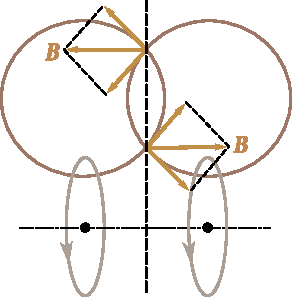
\includegraphics[scale=1]{figures/ch_06/fig_6_28.pdf}
			\caption[]{}
			\label{fig:6_28}
		\end{center}
	\end{minipage}
\vspace{-0.4cm}
\end{figure}

Vì vector $\vec{B}$ song song với trục solenoid nên từ trường bên trong cũng như bên ngoài cuộn phải là đồng nhất. Để chứng minh điều này, ta sẽ giả thiết có một vòng hình chữ nhật $1$-$2$-$3$-$4$ đặt bên trong cuộn (\fig{6_29}; $4$-$1$ hướng dọc theo trục của solenoid).

Chọn chiều quay quanh vòng kín là cùng chiều kim đồng hồ, ta sẽ có lưu số của $\vec{B}$ là $(B_2 - B_1)a$. Vòng kín ta chọn không chứa dòng điện, do vậy lưu số phải bằng không [từ \eqn{6_101}]. Từ đó ta suy ra $\vec{B}_1 = \vec{B}_2$. Ta thấy rằng khi ta thay đổi khoảng cách giữa đoạn $2$-$3$ của vòng kín trên với trục solenoid, ta luôn nhận được kết quả là $\vec{B}_2$ ở khoảng cách này bằng với $\vec{B}_1$ trên trục của solenoid. Nói cách khác, từ trường bên trong cuộn solenoid là đồng nhất.

Giờ ta hãy khảo sát vòng kín $1'$-$2'$-$3'$-$4'$. Ta sẽ kí hiệu $\vec{B}_1'$ và $\vec{B}_2'$ bằng nét gạch vì, như ta sẽ thấy sau đây, từ trường bên ngoài một solenoid vô hạn là bằng không. Ở trên, ta đã chứng minh rằng từ trường bên ngoài cuộn solenoid phải ngược chiều với từ trường bên trong cuộn. Vòng kín $1'$-$2'$-$3'$-$4'$ không chứa dòng điện; do vậy, lưu số của vector $\vec{B}'$ quanh vòng kín này bằng với $(B_1' - B_2')a$ và phải bằng không. Từ đây ta được $\vec{B}_1'=\vec{B}_2'$.
Khoảng cách từ trục của cuộn solenoid đến đoạn $1'$-$4'$ và $2'$-$3'$ được chọn bất kì. Do đó, giá trị của $\vec{B}'$ tại bất kì điểm nào nằm ngoài trục cũng sẽ như nhau. Vậy ta đã chứng minh được rằng từ trường bên ngoài cuộn là đồng nhất.

Lưu số quanh vòng kín trong hình \fig{6_30} là $a(B+B')$ (khi đi theo chiều kim đồng hồ). Vòng trên chứa dòng điện có độ lớn là $\ab{j}{lin}a$. Từ \eqn{6_101}, ta thu được phương trình sau:
\begin{equation*}
    a(B+B') = \mu_0 \ab{j}{lin} a,
\end{equation*}

\noindent
và sau khi loại bỏ $a$ ở hai vế và thay $\ab{j}{lin}$ bằng $nI$ [xem lại \eqn{6_106}]
\begin{equation}\label{eq:6_107}
    (B+B') = \mu_0 n I.
\end{equation}

\noindent
Phương trình trên cho thấy rằng từ trường ở cả bên trong và bên ngoài một solenoid dài vô tận là hữu hạn.

\begin{figure}[t]
	\begin{minipage}[t]{0.48\linewidth}
		\begin{center}
			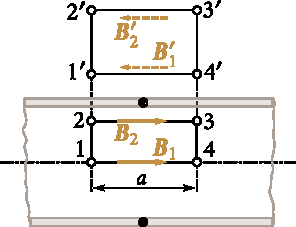
\includegraphics[scale=1]{figures/ch_06/fig_6_29.pdf}
			\caption[]{}
			\label{fig:6_29}
		\end{center}
	\end{minipage}
	\hfill{ }%space{-0.05cm}
	\begin{minipage}[t]{0.48\linewidth}
		\begin{center}
			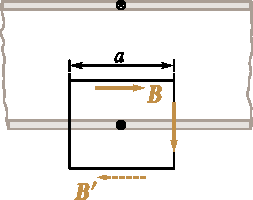
\includegraphics[scale=1]{figures/ch_06/fig_6_30.pdf}
			\caption[]{}
			\label{fig:6_30}
		\end{center}
	\end{minipage}
\vspace{-0.4cm}
\end{figure}

Chúng ta sẽ xét một mặt phẳng vuông góc với trục của solenoid (\fig{6_31}). Do các đường sức từ $\vec{B}$ kín nên từ thông qua mặt trong $S$ và mặt ngoài $S'$ của mặt phẳng trên phải là như nhau. Vì từ trường là đồng nhất và vuông góc với mặt phẳng được chọn vậy nên từ thông sẽ bằng độ lớn cảm ứng từ nhân với diện tích của phần có đường sức từ đi qua. Ta sẽ thu được hệ thức
\begin{equation*}
    BS = B'S'.
\end{equation*}

Vế trái của phương trình trên là hữu hạn trong khi đại lượng $S'$ ở vế phải lớn vô cùng nên ta suy ra $B'=0$.

Ta đã chứng minh được rằng cảm ứng từ bên ngoài một cuộn solenoid dài vô hạn bằng không. Từ trường bên trong cuộn là đồng nhất. Thay $B' = 0$ vào \eqn{6_107}, ta sẽ có được biểu thức cho cảm ứng từ bên trong solenoid:
\begin{equation}\label{eq:6_108}
    B = \mu_0 n I.
\end{equation}

Tích $nI$ được gọi là ampe-vòng trên mét. Với $n = 1000$ vòng trên mét và cường độ dòng điện có độ lớn \SI{1}{\ampere}, cảm ứng từ bên trong cuộn solenoid sẽ là $4\pi\times\SI{e-4}{\tesla}=4\pi \si{\gauss}$.

Các vòng được đặt đối xứng sẽ sinh ra từ trường tương tự trên trục của solenoid [xem lại \eqn{6_81}]. Do đó, ở đầu hở của một solenoid bán vô hạn, cảm ứng từ trên trục sẽ có giá trị bằng một nửa giá trị tính được trong \eqn{6_108}:
\begin{equation}\label{eq:6_109}
    B = \frac{1}{2} \mu_0 n I.
\end{equation}

Trên thực tế, nếu chiều dài của một solenoid lớn hơn đáng kể so với đường kính của nó thì \eqn{6_108} sẽ đúng với các điểm ở giữa cuộn, còn \eqn{6_109} sẽ đúng với các điểm ở trên trục và gần hai đầu của cuộn solenoid.

Toroid là một dây dẫn được quấn quanh một vật có hình xuyến (\fig{6_32}). Chúng ta hãy xem xét một vòng kín có dạng một đường tròn bán kính $r$ và có tâm trùng với tâm của toroid kể trên. Do tính đối xứng nên vector $\vec{B}$ tại mọi điểm phải có chiều tiếp tuyến với vòng kín. Vậy lưu số của $\vec{B}$ là
\begin{equation*}
    \oint \vec{B} \ccdot \derivec{l} = B \times 2\pi r
\end{equation*}

\noindent
($\vec{B}$ là cảm ứng từ ở những điểm thuộc vòng kín).

\begin{figure}[t]
	\begin{minipage}[t]{0.48\linewidth}
		\begin{center}
			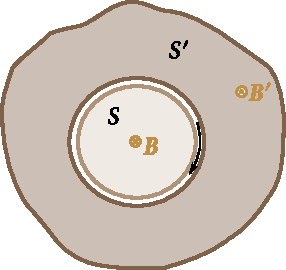
\includegraphics[scale=1]{figures/ch_06/fig_6_31.pdf}
			\caption[]{}
			\label{fig:6_31}
		\end{center}
	\end{minipage}
	\hfill{ }%space{-0.05cm}
	\begin{minipage}[t]{0.48\linewidth}
		\begin{center}
			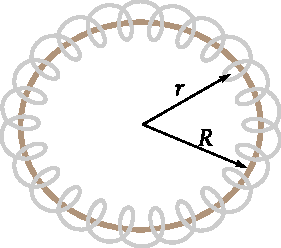
\includegraphics[scale=1]{figures/ch_06/fig_6_32.pdf}
			\caption[]{}
			\label{fig:6_32}
		\end{center}
	\end{minipage}
\vspace{-0.4cm}
\end{figure}

Nếu vòng kín nằm bên trong toroid, nó sẽ bao lấy dòng điện $2\pi RnI$ ($R$ là bán kính của toroid, còn $n$ là số vòng cuốn trên một đơn vị độ dài). Trong trường hợp này, ta sẽ có
\begin{equation*}
    B \times 2\pi r = \mu_0 2\pi R n I,
\end{equation*}

\noindent
từ đây ta được
\begin{equation}\label{eq:6_110}
    B = \mu_0 n I \frac{R}{r}.
\end{equation}

Nếu vòng kín nằm ngoài toroid, tổng dòng điện đi qua mặt của vòng sẽ là không và từ đó ta sẽ được $B\times 2\pi r = 0$. Vậy cảm ứng từ bên ngoài toroid bằng không.

Nếu toroid có bán kính $R$ lớn hơn rất nhiều so với bán kính của một vòng cuốn, tỉ số $R/r$ cho mọi điểm bên trong toroid sẽ xấp xỉ bằng một, và thay vì \eqn{6_110} thì ta sẽ thu được phương trình giống với \eqn{6_108} cho cuộn solenoid dài vô hạn. Trong trường hợp này, ta có thể coi từ trường trong toroid là đều. Tuy nhiên, vì từ trường bên trong cuộn toroid có hướng khác nhau ở các điểm khác nhau nên ta chỉ có thể nói rằng độ lớn của $\vec{B}$ là đồng nhất bên trong toàn bộ toroid.

Một cuộn toroid thật sẽ có thành phần dòng điện hướng dọc theo trục của nó. Thành phần dòng điện này sẽ sinh ra từ trường tương tự như từ trường tạo bởi dòng điện tròn ngoài thành phần từ trường được miêu tả trong \eqn{6_110}.
